% BU ECE template for MS thesis and PhD dissertation.
%
%==========================================================================%
% MAIN PREAMBLE 
%==========================================================================%
\documentclass[12pt,letterpaper]{report}          % Single-sided printing for the library
%\documentclass[12pt,twoside]{report} % Double-sided printing
\usepackage[intlimits]{amsmath}
\usepackage{multirow}
\usepackage{amsfonts,amssymb}
\usepackage{comment}
\usepackage{mathtools}
\usepackage{listings}
\usepackage{xcolor}
%\DeclareSymbolFontAlphabet{\mathbb}{AMSb}
%\usepackage{natbib}
\usepackage{apalike}
\usepackage{float}
\usepackage[bf]{caption}       
\setcaptionmargin{0.5in}
\usepackage{fancyhdr}
%\usepackage{fancyheadings}
\usepackage{fancybox}
\usepackage{ifthen}
\usepackage{bu_ece_thesis}
\usepackage{url}
\usepackage{lscape,afterpage}
\usepackage{xspace}
\usepackage{epstopdf} 
\usepackage{subfig}
\usepackage{multicol}
%==========================================================================%
%%% graphicx and pdf creation
\usepackage{graphicx}
\usepackage{appendix}
\DeclareMathOperator*{\argmax}{argmax} % thin space, limits underneath in displays

\definecolor{codegreen}{rgb}{0,0.6,0}
\definecolor{codegray}{rgb}{0.5,0.5,0.5}
\definecolor{codepurple}{rgb}{0.58,0,0.82}
\definecolor{backcolour}{rgb}{0.95,0.95,0.92}
 
\lstdefinestyle{mystyle}{
    backgroundcolor=\color{backcolour},   
    commentstyle=\color{codegreen},
    keywordstyle=\color{magenta},
    numberstyle=\tiny\color{codegray},
    stringstyle=\color{codepurple},
    basicstyle=\ttfamily\footnotesize,
    breakatwhitespace=false,         
    breaklines=true,                 
    captionpos=b,                    
    keepspaces=true,                 
    numbers=left,                    
    numbersep=5pt,                  
    showspaces=false,                
    showstringspaces=false,
    showtabs=false,                  
    tabsize=2
}
\lstset{style=mystyle}

%\usepackage{psfrag}
%\DeclareGraphicsExtensions{.eps}   % extension for included graphics
%\usepackage{thumbpdf}              % thumbnails for ps2pdf
%\usepackage[ps2pdf,                % hyper-references for ps2pdf
%bookmarks=true,%                   % generate bookmarks ...
%bookmarksnumbered=true,%           % ... with numbers
%hypertexnames=false,%              % needed for correct links to figures !!!
%breaklinks=true,%                  % breaks lines, but links are very small
%linkbordercolor={0 0 1},%          % blue frames around links
%pdfborder={0 0 112.0}]{hyperref}%  % border-width of frames 
%                                   % will be multiplied with 0.009 by ps2pdf
%\hypersetup{
%  pdfauthor   = {Joe Graduate <joe.graduate@bu.edu>},
%  pdftitle    = {dissertation.pdf},
%  pdfsubject  = {doctoral dissertations},
%  pdfkeywords = {mathematics, science, technology},
%  pdfcreator  = {LaTeX with hyperref package},
%  pdfproducer = {dvips + ps2pdf}
%}
%==========================================================================%
% customized commands can be placed here
%\newcommand{\figref}[1]{Figure~\ref{#1}}
%\newcommand{\chapref}[1]{Chapter~\ref{#1}}
%\newcommand{\latex}{\LaTeX\xspace}
%==========================================================================%

%==========================================================================%
% BEGIN
%==========================================================================%



\begin{document}

% The preliminary pages

% This file contains all the necessary setup and commands to create
% the preliminary pages according to the buthesis.sty option.

\title{Query planning for Stream Processing}

\author{Apoorva Tamaskar}

% Type of document prepared for this degree:
%   1 = Master of Science thesis,
%   2 = Doctor of Philisophy dissertation.
%   3 = Master of Science thesis and Doctor of Philisophy dissertation.
\degree=2

\prevdegrees{	M.Sc.,  University of Glasgow, 2018\\
B.Sc. Hons, Chennai Mathematical Institute , 2017}

\department{Department of Computer Science}

% Degree year is the year the diploma is expected, and defense year is
% the year the dissertation is written up and defended. Often, these
% will be the same, except for January graduation, when your defense
% will be in the fall of year X, and your graduation will be in
% January of year X+1
\defenseyear{2020}
\degreeyear{2020}

% For each reader, specify appropriate label {First, Second, Third},
% then name, and title. IMPORTANT: The title should be:
%   "Professor of Electrical and Computer Engineering",
% or similar, but it MUST NOT be:
%   Professor, Department of Electrical and Computer Engineering"
% or you will be asked to reprint and get new signatures.
% Warning: If you have more than five readers you are out of luck,
% because it will overflow to a new page. You may try to put part of
% the title in with the name.
\reader{First}{Kia Teymourian, PhD}{Assistant Professor of computer science}
\reader{Second}{Eugene Pinsky, PhD}{Assistant Professor of Computer Science}
\reader{Third}{Reza Rawassizadeh, PhD}{Associate Professor of Computer Science }

% The Major Professor is the same as the first reader, but must be
% specified again for the abstract page. Up to 4 Major Professors
% (advisors) can be defined. 
\numadvisors=1
\majorprof{Kia Teymourian, PhD}{{Assistant Professor of computer science}}
%\majorprofc{First M. Last, PhD}{{Professor of Astronomy}}
%\majorprofd{First M. Last, PhD}{{Professor of Biomedical Engineering}}

%%%%%%%%%%%%%%%%%%%%%%%%%%%%%%%%%%%%%%%%%%%%%%%%%%%%%%%%%%%%%%%%  

%                       PRELIMINARY PAGES
% According to the BU guide the preliminary pages consist of:
% title, copyright (optional), approval,  acknowledgments (opt.),
% abstract, preface (opt.), Table of contents, List of tables (if
% any), List of illustrations (if any). The \tableofcontents,
% \listoffigures, and \listoftables commands can be used in the
% appropriate places. For other things like preface, do it manually
% with something like \newpage\section*{Preface}.

% This is an additional page to print a boxed-in title, author name and
% degree statement so that they are visible through the opening in BU
% covers used for reports. This makes a nicely bound copy. Uncomment only
% if you are printing a hardcopy for such covers. Leave commented out
% when producing PDF for library submission.
%\buecethesistitleboxpage

% Make the titlepage based on the above information.  If you need
% something special and can't use the standard form, you can specify
% the exact text of the titlepage yourself.  Put it in a titlepage
% environment and leave blank lines where you want vertical space.
% The spaces will be adjusted to fill the entire page.
\maketitle
\cleardoublepage

% The copyright page is blank except for the notice at the bottom. You
% must provide your name in capitals.
\copyrightpage
\cleardoublepage

% Now include the approval page based on the readers information
\approvalpage
\cleardoublepage

% Here goes your favorite quote. This page is optional.
\newpage
%\thispagestyle{empty}

% \vspace{0.7in}
%
% \noindent
% [The descent to Avernus is easy; the gate of Pluto stands open night
% and day; but to retrace one's steps and return to the upper air, that
% is the toil, that the difficulty.]

\cleardoublepage

% The acknowledgment page should go here. Use something like
% \newpage\section*{Acknowledgments} followed by your text.
\newpage
\section*{\centerline{Acknowledgments}}
Over the course of writing this thesis, I have received lots of support and assistance.\\
First of all, I would like to thank my supervisor, Professor Kia Teymourian, who guided me and helped me formulate the research question, provided me with sources and methodology. Your insightful feedback pushed me to sharpen my thought process and helped me elevate the quality of my work.\\
I would like to thank the administrative staff at MET college, especially Ronette Lyle and the BU ISSO team who helped me through the administrative process.\\
I would like to acknowledge my friends and colleagues at Boston University for their wonderful feedback and discussions.\\
Also, I would like to thank my parents and my brother for their wise counsel, an empathetic ear and for always being there for me.
\vskip 1in

\noindent
Apoorva Tamaskar\\
Metropolitan College

\cleardoublepage

% The abstractpage environment sets up everything on the page except
% the text itself.  The title and other header material are put at the
% top of the page, and the supervisors are listed at the bottom.  A
% new page is begun both before and after.  Of course, an abstract may
% be more than one page itself.  If you need more control over the
% format of the page, you can use the abstract environment, which puts
% the word "Abstract" at the beginning and single spaces its text.

\begin{abstractpage}
% ABSTRACT
Our increasingly connected world has resulted in the generation of many data streams. With the rise in network traffic and increased interconnectivity, analyzing data and extracting key information has become challenging. Executing queries to extract insights from the data is now more essential than ever to make quick and efficient decisions. The flexibility of reinforcement learning, along with strong prediction properties, and precise mathematical model of Deep neural networks combined results in the technique called Deep reinforcement learning which can be a robust and promising method to reduce query processing times. While there is a lot of research on query optimization on data streams, none showcase the use of Deep reinforcement learning. The continuous nature of datastreams renders the conventional approaches inapplicable, due to increased processing time. The method implemented in this thesis is generic enough so that it applies to a wide range of data streams and queries to optimize the query processing time. The goal of this study is to act as a proof of concept. The thesis explores the use of deep reinforcement learning on a query from Linear road benchmark data. The proposed method is demonstrated to be effective in picking optimal query plan, and reducing the query execution time. We hope the work in this thesis encourages others to work on the development of a robust and more generalized system, capable of optimizing any query on any data stream.


\end{abstractpage}
\cleardoublepage

% Now you can include a preface. Again, use something like
% \newpage\section*{Preface} followed by your text

% Table of contents comes after preface
\tableofcontents
\cleardoublepage

% If you do not have tables, comment out the following lines
\newpage
\listoftables
\cleardoublepage

% If you have figures, uncomment the following line
\newpage
\listoffigures
\cleardoublepage

% List of Abbrevs is NOT optional (Martha Wellman likes all abbrevs listed)
\chapter*{List of Abbreviations}

{\bf The list below must be in alphabetical order as per BU library instructions or it will be returned to you for re-ordering.}

\begin{center}
  \begin{tabular}{lll}
    \hspace*{2em} & \hspace*{1in} & \hspace*{4.5in} \\
    CAD  & \dotfill & Computer-Aided Design \\
    CO   & \dotfill & Cytochrome Oxidase \\
    DOG  & \dotfill & Difference Of Gaussian (distributions) \\
    FWHM & \dotfill & Full-Width at Half Maximum \\
    LGN  & \dotfill & Lateral Geniculate Nucleus \\
    ODC  & \dotfill & Ocular Dominance Column \\
    PDF  & \dotfill & Probability Distribution Function \\
    $\mathbb{R}^{2}$  & \dotfill & the Real plane \\
  \end{tabular}
\end{center}
\cleardoublepage

% END OF THE PRELIMINARY PAGES

\newpage
\endofprelim
        
\cleardoublepage


\chapter{Introduction}
\label{chapter:Introduction}
\thispagestyle{myheadings}

\section{Motivation}
\label{sec:Motivation}
Hi
\section{Problem at hand}
\label{sec:Problem at hand}
Hello
\section{Structure of thesis}
\label{sec:Structure of thesis}
Works
\section{Conclusion}
\label{sec:Conclusion}
Nope

\cleardoublepage



\chapter{Related Work}
\label{chapter:related_work}
\thispagestyle{myheadings}

% set this to the location of the figures for this chapter. it may
% also want to be ../Figures/2_Body/ or something. make sure that
% it has a trailing directory separator (i.e., '/')!
\graphicspath{{2_Body/Figures/}}

\section{Introduction, Query optimization}
A database can be thought of as a list of tables, where in each table itself can be considered as a list of data points ordered initially in the sequence they are entered.
\par There are various tools which can be used to connect to a database, here we focus on structured query languages(SQL). A simple SQL query looks like this
\begin{lstlisting}[language=SQL]
    SELECT column_name_1, column_name_2
    FROM table_name
    WHERE condition
\end{lstlisting}
This query is essentially asking to display the 2 columns from the table where the condition given is satisfied. This to particular query might be looking simple, but if the condition introduced is a complex one or if the table from which we need to return the output is complex, the question of how to execute the query optimally becomes difficult to answer.

\section{Converting SQL queries to parse trees}
The exact grammar for the convertion to parse tree is not listed below. But this step isn't simply conversion to a parse tree, the preprocessor which does the conversion also has several more functions.
\par For example, if the SQL query uses a "view" in the query as a relation, then each instance has to be replaced by the parse tree.
\par The preprocessor also has to conduct semantic checking, that is, check if relations used exist, check for ambiguity, and type checking. If a parse tree passes the preprocessing then it is said to be \textbf{valid}.  In these parse trees, there are 2 types of nodes, one the atoms, which are essentially keywords in SQL, operators, constants and attributes. The second is Syntactic categories, these are names for families of subqueries in triangular brackets. Each of the syntactic category has unique expansion into atoms and further syntactic categories.


\section{Relational algebra}
As we saw above, order of operations matters, if the order of operations is not thoughtout and done blindly alot of redundant steps are executed and memory is moved around unnecessarily. There are few ways to atleast look and analyse the operations and how they can be simplied.
\par Let \textsc{R,S} be relations. Some simple laws, associativity and commutativity can easily be verified:-
\begin{itemize}
    \item $R\times S = S \times R$
    \item $(R\times S) \times T = R\times (S \times T)$
    \item $R \bowtie S = S \bowtie R$
    \item $(R \bowtie S) \bowtie T = R \bowtie (S \bowtie T)$
    \item $R \cup S = S \cup R$
    \item $(R \cup S) \cup T = R \cup (S \cup T)$
    \item $R \cap S = S \cap R$
    \item $(R \cap S) \cap T = R \cap (S \cap T)$
\end{itemize}
When applying associative law on relations, need to be careful whether the conditions actually makes sense after the order is changed.
\par While the above identities work on both sets and bags(bags allow for repeatition). To show that laws for sets and bags do differ an easy way is to consider the distributive property.
\begin{center}
$A\cap _S(B\cup_S C) = (A\cap_S B)\cup_S(A\cap_S C)$\\
$A\cap _B(B\cup_B C) \neq (A\cap_B B)\cup_B(A\cap_B C)$
\end{center}
We can simply show it with an example. Let $A=\{t\},B=\{t\},C=\{t\}$. The LHS comes to be $\{t\}$, whereas RHS is $\{t,t\}$

\subsection{Select operator $\sigma$}
First we start with simple properties of the $\sigma$ operator. Need to be careful about the attributes used in the select operator condition when pushing it down.
\begin{itemize}
    \item $\sigma_{C_1 \land C_2}(R) = \sigma_{C_1}(\sigma_{C_2}(R)) $
    \item $\sigma_{C_1 \lor C_2}(R) = (\sigma_{C_1}(R)) \cup_S (\sigma_{C_2}(R))$
    \item $\sigma_{C}(R \cup S) = \sigma_{C}(R) \cup \sigma_{C}(S)$
    \item $\sigma_{C}(R - S) = \sigma_{C}(R) - \sigma_{C}(S) = \sigma_{C}(R) - S$
    \item $\sigma_{C}(R \times S) = \sigma_{C}(R) \times S$
    \item $\sigma_{C}(R \bowtie S) = \sigma_{C}(R) \bowtie S$
    \item $\sigma_{C}(R \underset{D}{\bowtie} S) = \sigma_{C}(R) \underset{D}{\bowtie} S$
    \item $\sigma_{C}(R \cap S) = \sigma_{C}(R) \cap S$
\end{itemize}

\subsection{Projection operator $\pi$}
While for the Select operator($\sigma$) the identities were quite straight forward with not many things to consider, the identities for Projection operator ($\pi$) are bit more involved.
\begin{itemize}
    \item $\pi_{L}(R \bowtie S) = \pi_{L}(\pi_{M}(R) \bowtie \pi_{N}(S))$, where $M,N$ are attributes required for the join or they are inputs to the projection.
    \item $\pi_{L}(R \underset{D}{\bowtie} S) = \pi_{L}(\pi_{M}(R) \underset{D}{\bowtie} \pi_{N}(S))$, similar to above identity/ law.
    \item $\pi_{L}(R \times S) = \pi_{L}(\pi_{M}(R) \times \pi_{N}(S))$
    \item $\pi_{L}(R \cup_{B} S) = \pi_{L}(R) \cup_{B} \pi_{L}(S)$
    \item $\pi_{L}(\sigma_{C}(R))=\pi_{L}(\sigma_{C}(\pi_{M}(R))$
\end{itemize}

\subsection{Duplicate Elimination operator $\delta$}
The $\delta$ operator eliminates duplicates from bags. 
\begin{itemize}
    \item $\delta(R)= R,$ if $R$ does not have any duplicates.
    \item $\delta(R \times S) = \delta(R) \times \delta(S)$
    \item $\delta(R \bowtie S) = \delta(R) \bowtie \delta(S)$
    \item $\delta(R \underset{D}{\bowtie} S) = \delta(R) \underset{D}{\bowtie} \delta(S)$
    \item $\delta(\sigma_{C}(R)) = \sigma_{C}(\delta(R))$
    \item $\delta(R \cap_{B} S) = \delta(R) \cap_{B} S$
\end{itemize}

\subsection{Aggregation operator $\gamma$}
It is difficult to give identities for the aggregation operator, like done for the above operators. This is mostly due to how the details of how the aggregation operator is used.
\begin{itemize}
    \item $\sigma(\gamma_{L}(R)) = \gamma_{L}(R)$
    \item $\gamma_{L}(R) = \gamma_{L}(\pi_{M}(R)),$ where $M$ must at least contain the attributed used in $L$.
\end{itemize}


\section{Converting Parse trees into logical expression}
Till now, the only SQL related information presented is how to convert a Query into the parse tree, which is grammar dependent. Given the parse tree, need to substitute nodes by operators seen above, later this expression is optimized to be later converted to a physical query plan.
\par Now to convert the parse tree into the logical expression. First, look at the transformation of select-from-where statement.
\begin{itemize}
    \item $<Query> \rightarrow <SFW>.$
    \item $<SFW> \rightarrow SELECT <SelList> FROM <FromList> WHERE <Condition>.$
    \item $<SelList> \rightarrow \pi_{L}$, where $L$ is the list of attributes in $<SelList>.$
    \item $<Condition> \rightarrow \sigma_{C},$ where $C$ is the equivalent of $<Condition>$ 
\end{itemize}
While there is nothign inherently wrong about the last statement, need to consider the case where $<Condition>$ involves subqueries. A simple explanation about why it isn't allowed is a convention normally the subscript has to be a boolean condition, and if it was allowed otherwise, it would be a very expensive operation, as the subscript in the select operator has to evaluted at every element of the argument relation. This shows the redundance of it. While if this is allowed, it can be simplified and made efficient, but has to be done on a case by case basis with the use of $\bowtie, \times$ functions.
\par Overall it is a good idea to not use subquerying and rather using joins.
\par At this point, by making the substitutions mentioned above and using the algebraic identities, we obtain a starting logical query plan. The query has to be transformed into a query which the compiler believes to be the cheapest or the optimal. But, a thing which further complicates the process is the join order.
\par With the current knowledge, few optimizing rules are evident.
\begin{itemize}
    \item \textbf{Selection repositioning}, Selections should be pushed down as much as possbile, but sometimes, might need to take the selection operator a level up first.
    \item Pushing projections down the parse tree, being careful with the new projections made in the process.
    \item Duplicate removal needs to be repositioned.
    \item $\sigma$ combined with $\times$ below can result in equijoin, which is much more efficient. 
\end{itemize}
\par Normally, parsers only have nodes with $0, 1, 2$ children, which corresponds to uniary and binary operators. But many of the operators(natural join, union, and intersection) are commutative and associative, so it helps combine them on a single level to provide the opportunity to prioritize which ones are done first. To do this step, the following guidelines are sufficient.
\begin{itemize}
    \item We must replace the natural joins with theta-joins that equate the at­ tributes of the same name.
    \item We must add a projection to eliminate duplicate copies of attributes in­volved in a natural join that has become a theta-join
    \item The theta-join conditions must be associative.
\end{itemize}


\section{Explain difficulties/ Time complexity}
Currently, we have taken a query as an input and converted it into a logical plan, and then applied more transformation using relational algebra to make the optimal query plan. The next step is to convert it into a physical query plan which can be executed. To complete this step, need to compare the cost of various physical query plan derived from the logical query plan. This plan with the least cost is then passed query execution engine and executed. When trying to select a query plan, need to select:-
\begin{itemize}
    \item An order for the bracketing for associative and commutative operations like joins, unions, and intersections.
    \item The underlying algorithm for each operator in the logical plan, for instance, deciding whether a nested-loop join or a hash-join should be used.
    \item Need to consider additional operators like scanning, sorting, and so on that are needed for the physical plan but that were not present explicitly in the logical plan.
    \item A method for passing information/ variable values fromt the output of one operator to the next, for instance, by storing the intermediate result on disk or by using iterators and passing an argument one tuple or one main-memory buffer at a time.
\end{itemize}
Finally after selecting all these methods need to actually check the time required to excute the plan, one obivious way to calculate the time is actually executing the plan to see the cost. But if we try to find the optimal plan by this method then we are essentially executing every plan. That is expensive and redundant. The next few section presents few methods which can help in this task.

\subsection{Estimating size and cost}
$B(R) \coloneqq$ is the number of blocks needed to hold all the tuples of relation $R$.\\
$T(R) \coloneqq$ is the number of tuples of relation $R$.\\
$V(R,a) \coloneqq$ is the value count for attribute a of relation $R$, that is, the number of distinct values relation $R$ has in attribute $a$.\\
$V(R, [ a_1 , a_2,..., a_n]) \coloneqq$ is the number of distinct values $R$ has when all of attributes $a_1, a_2,..., a_n$ are considered together, that is, the number of tuples in $\delta(\pi_{a_1,a_2,...,a_n}(R))$
\par Compared to algorithms learnt in an introductory algorithms class, here the memory usage is huge and need to remember that intermidate/ temporary relations calculated will also incur a cost on the system. So need to take them into account as well because the physical plan is selected to minimize the estimated cost of evaluating the query. Over all the estimation method should pass the following sanity check:-
\begin{itemize}
    \item Give accurate estimates. No matter what method is used for executing query plans.
    \item Are easy to compute.
    \item Are logically consistent; that is, the size estimate for an intermediate re­lation should not depend on how that relation is computed. For instance, the size estimate for a join of several relations should not depend on the order in which we join the relations.
\end{itemize}
Even though there is no agreed upon method to do this, it does not matter because the goal is to help select a query plan and not to find the exact minimum cost. So even if the estimated cost is wrong, but if it is wrong similarly then we will still have the least costing plan.

\subsection{Estimation of Projection}
The projection operator is a bag operation, so it does not reduce the number of tuples, only reduces the size of each tuple.\\
$T(R) = T(\pi(R))$\\
$B(R) \leq B(\pi(R))$

\subsection{Estimation of Selection}
Let $S = \sigma_{A=c}(R)$, here $A$ is an attribute of $R$ and $c$ is a constant\\
$T(S)=\frac{T(R)}{V(R,A)}$, is it important to note that this is an estimate and not the actual value, this will be the actual value if all the attributes in $A$ have equal occurance. An even better estimate can be obtained if the DBMS stores a statistic know as histogram. 
\par The above calculate was easy because of the equality. if $S=\sigma_{A < c}(R)$, we simply estimate $T(S)=\frac{T(R)}{3}$
\par Now if $S=\sigma_{A\neq c}(R)$, can take $T(S)=T(R)$ or $T(S)= T(R) - \frac{T(R)}{V(R,A)}$
\par If $S=\sigma_{A = c_1 \lor c_2}$, take them to be independent conditions.

\subsection{Estimation of Join, single attribute}
For natural joins, we assume, the natural join of two relations involves only the equality of two attributes. That is, we study the
join $R(X, Y) \bowtie S(Y, Z)$ , but initially we assume that $Y$ is a single attribute although X and Z can represent any set of attributes. But it is hard to find a good estimate as $T(R\bowtie S) \in [0, T(R)*T(S)]$, to help with this two assumptions are made.
\begin{itemize}
    \item \textbf{Containment of Value Sets} If Y is an attribute appearing in several rela­tions, then each relation chooses its values from the front of a fixed list of values $y_1, y_2, y_3,...$ and has all the values in that prefix. As a consequence, if $R$ and $S$ are two relations with an attribute $Y$, and $V(R, Y) \leq V(S, Y)$, then every $Y$-value of $R$ will be a $Y$-value of $S$. 
    \item \textbf{Preservation of Value Sets} If we join a relation $R$ with another relation, then an attribute A that is not a join attribute (i.e., not present in both relations) does not lose values from its set of possible values. More precisely, if $A$ is an attribute of $R$ but not of $S$, then $V(R \bowtie S, A) = V(R, A)$. Note that the order of joining $R$ and $S$ is not important, so we could just as well have said that $V(S \bowtie R, A) = V (R, A)$.
\end{itemize}
\par Using the above assumptions we can claim, 
$$T(R\bowtie S)=\frac{T(R)*T(S)}{max(V(R,Y), V(S,Y))}$$
Let $V(R,Y) \leq V(S,Y)$, then every tuple $t$ of $R$ has a chance of $\frac{1}{V(S,Y)}$ of joining with a given tuple of $S$. Since there are $T(S)$ tuples in $S$, the expected number of tuples that $t$ joins with is $\frac{T(S)}{V(S, Y)}$. As there are
$T(R)$ tuples of $R$, the estimated size of $R \bowtie S$ is $\frac{T(R)*T(S)}{V(S,Y)}$, if it was $V(R,Y) \geq V(S,Y)$, then $\frac{T(R)*T(S)}{V(R,Y)}$
\par Guidelines for other type of joins:-
\begin{itemize}
    \item The number of tuples in the result of an equijoin can be computed exactly as for a natural join, after accounting for the change in variable names.
    \item Other theta-joins can be estimated as if they were a selection following a product.
\end{itemize}

\subsection{Estimation of Join, multiple attribute}
Now we assume $Y$ in $R(X, Y) \bowtie S(Y, Z)$ represents multiple attributes. Say for example, $R(X, y_1, y_2) \bowtie S(y_1, y_2, Z)$. We again do a probability calculation.
\par Let $r \in R, s \in S$ be a tuples, the probability that $r,s$ agree on $y_1$ is $\frac{1}{max(V(R,y_1), V(S,y_1))}$, similarly for $y_2$. So we get the expected value to be
$$\frac{T(R)*T(S)}{max(V(R,y_1), V(S,y_1))*max(V(R,y_2), V(S,y_2))}$$ 
From this the pattern is clear, need to divide $T(R)*T(S)$ by maximum of $V(R,y), V(S,y)$ for each attribute.
\par But this is only the calculation for $T(R\bowtie S)$, need to calculate for $B(R\bowtie S)$ as well.

\subsection{Multiple Joins}
For this case we work with $S = R_1 \bowtie R_2 \bowtie ... \bowtie R_n$
\par Here we have to make use of the containment assumption. Say the attribute $A$ appears in $k$ of $R_i$'s and the values corresponding to $V(R_i,A)$ are $v_1 \leq v_2 \leq ... \leq v_k$, need to find the probability that tuples agree on $A$.
\par Consider the tuple $t_1$ chosen from the relation that has the small­est number of $A-$values, $v_1$ . By the containment assumption, each of these $v_1$ values is among the $A-$values found in the other relations that have attribute $A$. Consider the relation that has $V_i$ values in attribute $A$. Its selected tuple $t_i$ has probability $\frac{1}{v_1}$ of agreeing with $t_1$ on $A$. Since this claim is true for all $i \in \{2, 3,..., k\}$, the probability that all $k$ tuples agree on $A$ is the product $\frac{1}{v_2 * v_3 *...* V_k}$. This analysis gives us the rule for estimating the size of any join.
\par Start with the product of the number of tuples in each relation. Then for each attribute A appearing at least twice, divide by all but the least of the $V(R, A)$'s

\subsection{Union}
If $U_B$ is used, it is the sum of the two individually. 
\par If $U_S$ is used, then number of tuples range from the max of two, to their sum. So take mean of the range.

\subsection{Intersection}
The number of tuples here ranges from $0$ to the minimum of the two(in case of set intersection), so again can take the mean of this range.

\subsection{Difference}
The range for $R-S$ is $[T(R)-T(S),T(R)]$, so again mean of the range.

\subsection{Duplicate Elimination}
The range for $\delta(R)$ is $[1, T(R)]$, so again can take the mean, there can be other estimates as well.
\par A nice compromise is $min(\frac{T(R)}{2}, \prod V(R,a_i))$

\subsection{Grouping and Aggregation}
Same as duplicate.


\section{Other tools}
We assume that the "cost" of evaluating an expression is approximated well by the number of disk I/O's performed. The number of disk I/O's, in turn, is influenced by:
\begin{itemize}
    \item The particular logical operators chosen to implement the query.
    \item The sizes of intermediate results, need to pass them to the next function.
    \item The physical operators used to implement logical operators, e.g., the choice of a one-pass or two-pass join, or the choice to sort or not sort a given relation.
    \item The ordering of similar operations, especially joins.
    \item The method of passing arguments from one physical operator to the next.
\end{itemize}

\subsection{Histogram}
In the earlier section the statistics were heavily used in calculations. Another statistic that can be stored is the histogram.
\par If $V (R, A)$ is not too large, then the histogram may consist of the number (or fraction) of the tuples having each of the values of attribute $A$. If there are a great many values of this attribute, then only the most frequent values may be recorded individually, while other values are counted in groups.
\par \textbf{Equal width} To start, select 2 parameters, $w$ the width and $v_0$ a begining point of a column in the histogram, which will initally be the considered the lower bound and if an even lower value is noticed, make a smaller column as well and update the lower bound.
\par \textbf{Equal height} These are the common "percentiles". A percentile $p, 2p$, so on.
\par \textbf{Most frequent values} List the most common values and their numbers of occurrences. This information may be provided along with a count of occurrences for all the other values as a group, or we may record frequent values in addition to an equal width or equal height histogram for the other values.

\subsection{Heuristics}
One important use of cost estimates for queries or subqueries is in the appli­cation of heuristic transformations of the query.
\par Heuristics applied independent of cost estimates can be expected almost certainly to improve the cost of a logical query plan
\par However, there are other points in the query optimization process where es­timating the cost both before and after a transformation will allow us to apply a transformation where it appears to reduce cost and avoid the transformation otherwise. In particular, when the preferred logical query plan is being generated, we may consider a number of optional transformations and the costs before and after. Because we are estimating the cost of a logical query plan, so we have not yet made decisions about the physical operators that will be used to implement the operators of relational algebra, our cost estimate cannot be based on disk I / O's. Rather, we estimate the sizes of all intermediate results their sum is our heuristic estimate for the cost of the entire logical plan.

\section{Enumeration Methods}
The naive method of find the least costing plan is enumerating all the possible plans and calculating the cost for them and then selecting the minimum one.
\par \textbf{Top-Down} Here, we work down the tree of the logical query plan from the root. For each possible implementation of the operation at the root, we consider each possible way to evaluate its argument(s) , and compute the cost of each combination, taking the best.
\par \textbf{Bottom-up} For each subexpression of the logical-query-plan tree, we com­pute the costs of all possible ways to compute that subexpression. The possibilities and costs for a subexpression E are computed by consider­ing the options for the subexpressions for E , and combining them in all possible ways with implementations for the root operator of E.
\par There is actually not much difference between the two approaches in their broadest interpretations, since either way, all possible combinations of ways to implement each operator in the query tree are considered. When limiting the search, a top-down approach may allow us to eliminate certain options that could not be eliminated bottom-up. However, bottom-up strategies that limit choices effectively have also been developed. there is an apparent simplification of the bottom-up method, where we consider only the best plan for each subexpression when we compute the plans for a larger subexpression. This approach, called \textbf{dynamic programming}, is not guaranteed to yield the best plan, although often it does. The approach called Selinger-style (or System-R-style) optimization exploits additional properties that some of the plans for a subexpression may have, in order to produce optimal overall plans from plans that are not optimal for certain subexpressions.

\subsection{Heuristic Selection}
One option is to use the same approach to selecting a physical plan that is generally used for selecting a logical plan: make a sequence of choices based on heuristics. Few common ones are:-
\begin{itemize}
    \item If the logical plan calls for a selection  $\sigma_{A=c}(R)$, and stored relation R has an index on attribute A, then perform an index-scan to obtain only the tuples of $R$ with $A-$value equal to $c$.
    \item if the selection involves one condition like A = c above, and other conditions as well, we can implement the selection by an index­ scan followed by a further selection on the tuples, which we shall represent by the physical operator filter.
    \item If an argument of a join has an index on the join attribute(s), then use an index-join with that relation in the inner loop.
    \item If one argument of a join is sorted on the join attribute(s) , then prefer a sort-join to a hash-join, although not necessarily to an index-join if one is possible.
    \item When computing the union or intersection of three or more relations, group the smallest relations first.
\end{itemize}

\subsection{Branch-and-Bound}
This approach, often used in practice, begins by using heuristics to find a good physical plan for the entire logical query plan. Let the cost of this plan be $C$. Then as we consider other plans for subqueries, we can eliminate any plan for a sub query that has a cost greater than $C$, since that plan for the sub query could not possibly participate in a plan for the complete query that is better than what we already know. Likewise, if we construct a plan for the complete query that has cost less than $C$, we replace $C$ by the cost of this better plan in subsequent exploration of the space of physical query plans. An important advantage of this approach is that we can choose when to cut off the search and take the best plan found so far. For instance, if the cost $C$ is small, then even if there are much better plans to be found, the time spent finding them may exceed $C$, so it does not make sense to continue the search. However, if $C$ is large, then investing time in the hope of finding a faster plan is wise.

\subsection{Hill Climbing}
This approach, in which we really search for a "valley" in the space of physical plans and their costs, starts with a heuristically selected physical plan. We can then make small changes to the plan, e.g., replacing one method for an operator by another, or reordering joins by using the associative and/or commutativen laws, to find "nearby" plans that have lower cost. When we find a plan such that no small modification yields a plan of lower cost, we make that plan our chosen physical query plan .

\subsection{Selinger-Style Optimization}
This approach improves upon the dynamic-programming approach by keeping for each subexpression not only the plan of least cost, but certain other plans that have higher cost, yet produce a result that is sorted in an order that may be useful higher up in the expression tree. Examples of such interesting orders are when the result of the subexpression is sorted on one of:
\begin{itemize}
    \item The attribute(s) specified in a sort operator $(\tau)$ at the root.
    \item The grouping attribute(s) of a later group-by operator $(\gamma)$.
    \item The join attribute(s) of a later join. 
\end{itemize}
If we take the cost of a plan to be the sum of the sizes of the intermediate relations, then there appears to be no advantage to having an argument sorted. However, if we use the more accurate measure, disk I/O's, as the cost, then the advantage of having an argument sorted becomes clear if we can use one of the sort-based algorithms and save the work of the first pass for the argument that is sorted already.

\section{Join Order}
Join takes in two argument, while the end result is independent of the order of the two arguments, the method used to compute the result maybe dependent on the order. Perhaps most important, the one-pass join reads one relation preferably the smaller
into main memory, creating a structure such as a hash table to facilitate matching of tuples from the other relation. It then reads the other relation, one block at a time, to join its tuples with the tuples stored in memory. 
\par For instance, suppose that when we select a physical plan we decide to use a one-pass join. Then we shall assume the left argument of the join is the smaller relation and store it in a main-memory data structure. This relation is called the build relation. The right argument of the join, called the probe relation, is read a block at a time and its tuples are matched in main memory with those of the build relation. Other join algorithms that distinguish between their arguments include:
\begin{itemize}
    \item Nested-loop join, where we assume the left argument is the relation of the
outer loop.
    \item Index-join, where we assume the right argument has the index.
\end{itemize}

\subsection{Join Trees}
When we have the join of two relations, we need to order the arguments. We shall conventionally select the one whose estimated size is the smaller as the left argument. Notice that the algorithms mentioned above -- one-pass, nested­ loop, and indexed - each work best if the left argument is the smaller. More precisely, one-pass and nested-loop joins each assign a special role to the smaller relation (build relation, or outer loop), and index-joins typically are reasonable choices only if one relation is small and the other has an index. It is quite common for there to be a significant and discernible difference in the sizes of arguments, because a query involving joins very often also involves a selection on at least one attribute, and that selection reduces the estimated size of one of the relations greatly.
\par When we need to join more than $2$ relations, the order in which they are joined can be represented by a binary tree, where each node has either $0$ or $2$ children. A tree where the right child always a leaf node is called a left deep tree, one can similarly define a right deep tree. Any other tree is will be called \textbf{bushy}. We will stick with left deep tree due to their interaction with various common join algorithms. This introduced limitation also helps to reduce search space.
\par If one-pass joins are used, and the build relation is on the left, then the amount of memory needed at any one time tends to be smaller than if we used a right-deep tree or a bushy tree for the same relations.
\par If we use nested-loop joins, with the relation of the outer loop on the left, then we avoid constructing any intermediate relation more than once.

\subsection{DP to decide join order}
Suppose we need to calculate $R_1 \bowtie R_2 \bowtie ... \bowtie R_n$. For the DP algorithm construct a table with an entry for each subset of one or more of the n relations. In that table we put 
\begin{itemize}
    \item the estimated size of the join of these relations.
    \item the least cost of computing the join of these relations. Other, more complex estimates, such as total disk I/O's, could be used if we were willing and able to do the extra calculation involved.
    \item The expression that yields the least cost. This expression joins the set of relations in question, with some grouping. We can optionally restrict ourselves to left-deep expressions, in which case the expression is just an ordering of the relations.
\end{itemize}

\subsection{Greedy algorithm for join order}
Even the carefully limited search of dynamic pro­gramming leads to a number of calculations that is exponential in the number
of relations joined. It is reasonable to use an exhaustive method like dynamic programming or branch-and-bound search to find optimal join orders of five or six relations. However, when the number of joins grows beyond that, or if we choose not to invest the time necessary for an exhaustive search, then we can use a join-order heuristic in our query optimizer.
\par The most common choice of heuristic is a greedy algorithm, where we make one decision at a time about the order of joins and never backtrack or reconsider decisions once made. We shall consider a greedy algorithm that only selects a left-deep tree. The "greediness" is based on the idea that we want to keep the intermediate relations as small as possible at each level of the tree.
\par Start with the pair of relations whose estimated join size is smallest. The join of these relations becomes the current tree. Find, among all those relations not yet included in the current tree, the relation that, when joined with the current tree, yields the relation of smallest estimated size. The new current tree has the old current tree as its left argument and the selected relation as its right argument.


\section{Physical Query Plan}
We have parsed the query, converted it to an initial logical query plan, and improved that logical query plan with transformations. Part of the process of selecting the physical query plan is enumeration and cost­ estimation for all of our options, then focused on the question of enumeration, cost estimation, and ordering for joins of several relations. By extension, we can use similar techniques to order groups of unions, intersections, or any associative/commutative operation
\par There are still several steps needed to turn the logical plan into a complete
physical query plan.
\begin{itemize}
    \item Selection of algorithms to implement the operations of the query plan,
when algorithm-selection was not done as part of some earlier step such
as selection of a join order by dynamic programming.
    \item Decisions regarding when intermediate results will be materialized ( cre­
ated whole and stored on disk) , and when they will be pipelined (created
only in main memory, and not necessarily kept in their entirety at any
one time) .
    \item Notation for physical-query-plan operators, which must include details
regarding access methods for stored relations and algorithms for imple­
mentation of relational-algebra operators.
\end{itemize}

\subsection{Choosing a Selection Method}
One of the important steps in choosing a physical query plan is to pick algo­rithms for each selection operator.
\par Assuming there are no multidimensional indexes on several of the attributes,
then each physical plan uses some number of attributes that each have an index, and are compared to a constant in one of the terms of the selection. We then use these indexes to identify the sets of tuples that satisfy each of the
conditions. For simplicity, we shall not consider the use of several indexes in this way. Rather, we limit our discussion to physical plans that:
\begin{itemize}
    \item Use one comparison of the form $A\theta c$, where $A$ is an attribute with an index, $c$ is a constant, and $\theta$ s a comparison operator such as $=$ or $<$.
    \item Retrieve all tuples that satisfy the comparison, using the index­ scan physical operator.
    \item Consider each tuple selected to decide whether it satisfies the rest of the selection condition. We shall call the physical operator that per­forms this step Filter; it takes the condition used to select tuples as a parameter, much as the rr operator of relational algebra does.
\end{itemize}
In addition to physical plans of this form, we must also consider the plan that uses no index but reads the entire relation (using the table-scan physical oper­ator) and passes each tuple to the Filter operator to check for satisfaction of the selection condition. 
\par We decide among the physical plans with which to implement a given selec­tion by estimating the cost of reading data for each possible option. To compare costs of alternative plans we cannot continue using the simplified cost estimate of intermediate-relation size. The reason is that we are now considering imple­mentations of a single step of the logical query plan, and intermediate relations are independent of implementation. Thus, we shall refocus our attention and resume counting disk I/O's.

\subsection{Choosing a Join Method}
On the assumption that we know (or can estimate) how many buffers are available to perform the join, we can apply the formulas for sort/ indexed/ hash join. However, if we are not sure of, or cannot know, the number of buffers that will be available during the execution of this query (because we do not know what else the DBMS is doing at the same time), or if we do not have estimates of important size parameters such as the V (R, a)'s, then there are still some principles we can apply to choosing a join method. Similar ideas apply to other binary operations such as unions, and to the full-relation, unary operators, $\gamma, \delta$


\subsection{Pipelining Versus Materialization}
The last major issue we shall discuss in connection with choice of a physical query plan is pipelining of results. The naive way to execute a query plan is to order the operations appropriately (so an operation is not performed until the argument(s) below it have been performed), and store the result of each operation on disk until it is needed by another operation. This strategy is called materialization, since each intermediate relation is materialized on disk. A more subtle, and generally more efficient, way to execute a query plan is to interleave the execution of several operations. The tuples produced by one operation are passed directly to the operation that uses it, without ever storing the intermediate tuples on disk. This approach is called pipelining, and it typically is implemented by a network of iterators whose functions call each other at appropriate times. Since it saves disk I/O 's, there is an obvious advantage to pipelining, but there is a corresponding disadvan­tage. Since several operations must share main memory at any time, there is a chance that algorithms with higher disk-I/O requirements must be chosen , or thrashing will occur, thus giving back all the disk-I/O savings that were gained by pipelining, and possibly more.


\subsection{Pipelining Unary Operations}
Unary operations - selection and projection - are excellent candidates for pipelining. Since these operations are tuple-at-a-time, we never need to have more than one block for input, and one block for the output. We may implement a pipelined unary operation by iterators, The consumer of the pipelined result calls \textbf{GetNext()} each time another tuple is needed. In the case of a projection, it is only necessary to call \textbf{GetNext()} once on the source of tuples, project that tuple appropriately, and return the result to the consumer. For a selection $\sigma_C$ (technically, the physical operator \textbf{Filter(C)} ) , it may be necessary to call \textbf{GetNext()} several times at the source, until one tuple that satisfies condition $c$ is found.


\subsection{Pipelining Binary Operations}
The results of binary operations can also be pipelined. We use one buffer to pass the result to its consumer, one block at a time. However, the number of other buffers needed to compute the result and to consume the result varies, depending on the size of the result and the sizes of other relations involved in the query. We shall use an extended example to illustrate the tradeoffs and opportunities.


\subsection{Notation for Physical Query Plans}

\par \textbf{Operators for Leaves}
\par Each relation R that is a leaf operand of the logical-query-plan tree will be replaced by a scan operator. The options are:
\begin{itemize}
    \item \textbf{TableScan(R):} All blocks holding tuples of R are read in arbitrary order.
    \item \textbf{SortScan(R,L):} Tuples of R are read in order, sorted according to the attribute(s) on list L.
    \item \textbf{IndexScan(R,C):} Here, C i s a condition of the form $A\theta c$, where A is an attribute of $R, \theta$ is a comparison such as $=$ or $<$ , and $c$ is a constant. Tu­ples of $R$ are accessed through an index on attribute $A$. If the comparison $\theta$ is not $=$, then the index must be one, such as a B-tree, that supports range queries.
    \item \textbf{IndexScan(R,A):} Here $A$ is an attribute of $R$. The entire relation $R$ is retrieved via an index on $R.A.$ This operator behaves like \textbf{TableScan}, but may be more efficient in certain circumstances, if $R$ is not clustered and/or its blocks are not easily found.
\end{itemize}

\par \textbf{Physical Operators for Selection}
\par A logical operator $\sigma_C(R)$ is often combined, or partially combined, with the access method for relation $R$, when $R$ is a stored relation. Other selections, where the argument is not a stored relation or an appropriate index is not available, will be replaced by the corresponding physical operator we have called \textbf{Filter}.

\par \textbf{Physical Sort Operators}
\par Sorting of a relation can occur at any point in the physical query plan. We have already introduced the \textbf{SortScan(R, L)} operator, which reads a stored relation $R$ and produces it sorted according to the list of attributes $L$. When we apply a sort-based algorithm for operations such as join or grouping, there is an initial phase in which we sort the argument according to some list of attributes. It is common to use an explicit physical operator $Sort(L)$ to perform this sort on an operand relation that is not stored. This operator can also be used at the top of the physical-query-plan tree if the result needs to be sorted because of an \textbf{ORDER BY} clause in the original query,

\par \textbf{Other Relational-Algebra Operations}
\par All other operations are replaced by a suitable physical operator. These oper­ators can be given designations that indicate:
\begin{itemize}
    \item The operation being performed, e.g., join or grouping.
    \item Necessary parameters, e.g., the condition in a theta-join or the list of elements in a grouping.
    \item A general strategy for the algorithm: sort-based, hash-based, or in some joins, index-based.
    \item A decision about the number of passes to be used: one-pass, two-pass, or multipass (recursive, using as many passes as necessary for the data at hand) . Alternatively, this choice may be left until run-time.
    \item An anticipated number of buffers the operation will require.
\end{itemize}
\subsection{Ordering of Physical Operations}
Our final topic regarding physical query plans is the matter of order of oper­ations. The physical query plan is generally represented as a tree, and trees imply something about order of operations, since data must flow up the tree.However, since bushy trees may have interior nodes that are neither ancestors nor descendants of one another, the order of evaluation of interior nodes may not always be clear. Moreover, since iterators can be used to implement opera­tions in a pipelined manner, it is possible that the times of execution for various nodes overlap, and the notion of "ordering" nodes makes no sense. 
\par If materialization is implemented in the obvious store-and-later-retrieve way, and pipelining is implemented by iterators, then we may establish a fixed se­quence of events whereby each operation of a physical query plan is executed.The following rules summarize the ordering of events i m pl icit in a phy sical query-plan tree:
\begin{itemize}
    \item Break the tree into subtrees at each edge that represents materialization. The subtrees will be executed one-at-a-time.
    \item Order the execution of the subtrees in a bottom-up, left-to-right manner. To be precise, perform a preorder traversal of the entire tree. Order the subtrees in the order in which the preorder traversal exits from the subtrees.
    \item Execute all nodes of each subtree using a network of iterators. Thus, all the nodes in one subtree are executed simultaneously, with GetNext calls among their operators determining the exact order of events.
\end{itemize}

\section{Introduction to Data Streams}
A \textbf{Data Stream} can be thought of as a continuously generated never ending sequence of data. For example, network logistics, healthcare monitoring information, security cameras, all of these continuously produce data, these data sequences/ streams are crucial to their respective users/ organisations, realtime detection of anomally, pattern or changes thereof, or any other type of analytics is in need currently.
\par But there are many complications while trying to do this, the frequency of data generation isn't stable as it can keep changing throughout the cycle. Most of these service have a Quality of Service (or QoS) requirements defined which takes into account various metrics such as response time, memory usage, and throughput and more. Sometimes these requirements are so heavy and indulgent that it is infeasible to load the incoming data streams into a persistent store and process them effectively using DBMS tools. Hence special tools are required for these, similar to how DBMS has a variety of steps, Data Stream Management Systems (DSMSs) have multiple steps as well processing of sensor data, pervasive computing, situation monitoring, real-time response, approximate algorithms, on-the-fly mining, complex event processing, and more. While it may seem that optimizing Data stream applications to their specific domains may make them difficult to study, it is possible the generalize the functions/ steps enough to have a basic architecture to study.
\par Queries used in traditional DBMS are called \textbf{ad hoc queries}, where are the queries used in DSMS are called \textbf{ContinuousQueries (CQ)}. Ad hoc queries are generally specified, optimized, and evaluated over a snapshot of a database. Whereas, CQs are specified once and evaluated repeatedly against new data over a specified life span or as long as there exists data in the stream. They are long-running queries that produce output continuously. The result is also assumed to be a stream possibly with differing rates and schema (as compared to the input). The difference between ad hoc queries and CQs can be best understood based on their relationship to the data over which they are processed. Different or changing ad hoc queries are processed over (relatively) static data in contrast to the same (or static) CQs that are processed repeatedly over frequently changing (or dynamic) data. It is clear that DBMS can't really cope with data streams in terms on high frequency updates, fulfilling QoS and continuous output. Hence we make use of Data Stream Management Systems (DSMSs).


\section{Windowing and QoS}
Most of the languages used for this are based on SQL, some of them are,  Continuous Query Language (CQL), StreamSQL and ESP. Typically, continuous queries consist of relational operators 3 such as select, project, join, and other aggregation operators. A logical query plan, analogous to a query tree used in a traditional DBMS, can be generated from the specification of a CQ. It can then be transformed into a query plan consisting of detailed algorithms used for computing each operator. Compared to DBMS where either pipelines or materialization is used, DSMS use a push or dataflow methodology. All operators in a DSMS compute on data items as they arrive and cannot assume the stream to be finite. This has significant implications for the computation of a number of operators such as join, sort, and some aggregation operators. These operations cannot be completed without processing the entire input data set (or sets) which poses problems due to the unbounded nature of streams. As a result, these operators will block and produce no output until the stream ends. Hence, they are termed blocking operators. For an operator to output results continuously (and hopefully smoothly) and not wait until the end of the stream, it is imperative that these blocking operators be converted into non-blocking ones. The notion of a window has been introduced to overcome the blocking aspect of a number of operators. Informally, a window defines a finite portion of the stream (as a relation) for processing purposes. A window specification, added to a continuous query specification, can produce time-varying, finite relations out of a stream.
\par QoS management is important and critical to the success of a DSMS. Few of the popular QoS metrices are Tuple latency, Memory usage, Throughput, Smooth or bursty nature of output streams, Accuracy of results in terms of error tolerance. Most of the metrices can be specified in the query written. Overall to correlate CQs and QoS a simple question can be asked 
\begin{center}
Given a set of CQs with their QoS specifications, what resources are needed to compute the given CQs and satisfy their QoS requirements?
\end{center}

\section{Challenges of query optimization on data streams}
Picking up on the question form the last section, it is important to be able to address the inverse as well, i.e. given resources, CQs and QoS, need to verify that QoS are satisfied. Like any verification, there are two general ways of tackling this problem.
\begin{itemize}
    \item Try to model the load generated by the input stream and get a conservative estimate on the metrices used to measure the QoS.
    \item Continuously monitor the metrices while the program is running, on violation identify the bottleneck and improve upon it.
\end{itemize}
As seen in previous chapters, creating a model to predict the load can be very difficult and sometimes more expensive than the best result. So we focus on the second approach.

\subsection{Resource Scheduling Strategies}
Similar to the case of traditional DBMS, querying in DSMS involves multiple steps as well. The resource requirements for each step varies hence the need for a scheduling method which can determine an optimal schedule. To further complicate this, the various types of CQs have different QoS, hence the wiggle room for the performance is high, and as DSMS process queries in real time more considerations have to taken into account compared to traditional data bases, e.g. different operators require different amount of memory and time to process data. 

\subsection{Load Shedding and Run-Time Optimization}
It is important to note that optimizing resource allocation using any state of the art strategy does not guarantee that resources will be sufficient, as there might be some points in the data stream which overloads particular query, hence wiggle room in the performance/ accuracy, i.e. some of the data can be discarded to decrease the quality of the result and give an approximate result. This process of decreasing quality of result by not considering some tuple is called load shedding. Given that discarding tuples of the data stream is allowed, how do we decide which ones to discard? 

\subsection{Complex Event and Rule Processing}
In the first section we said we proceed with the second strategy, i.e. monitor the metrics. Can extend that idea further to monitor the output of CQs to detect anomalies. Initially, Comple Event Processing was not a part of DSMS, but now many models have been developed to integrate the two. With the integration comes many additional functionalities and helps develop a theoretical base, but also puts additional burden on the system. This along with run time optimiations makes the implementation of DSMS quite complicated.

\section{Deep Learning}
We expand on linear regression model. Given $\{(x^{(i)},y^{(i)})\}_{i=1}^{n}$ as data points, the goal is to find a function $h_{\theta}(x)$ which is "as close as possible" to $y_i$.
\par One way to do that is, define a loss function $J$ which measures the distance between prediction and actual value of $y^{(i)}$ as
$$J^{(i)}(\theta)=\frac{1}{2}(h_{\theta}(x^{(i)})-y^{(i)})^{2}$$
$$J(\theta)=\frac{1}{n}\sum_{i=1}^{n}J^{(i)}(\theta)$$
The goal then reduces to finding parametrize $h_{\theta}$ and finding the $\theta$ so that $J(\theta)$ is minimized.
\par Similarly in neural networks, we define a parameterization of $h$ and then try to minimize the loss function.
\par Consider the simplest neural network, which consists of an input layer and a output layer with a single neuron. Say, the input is $x$, then the output neuron has input $h_{\theta}(x)$, and the output from the neuron is $A(h_{\theta}(x))$, where $A$ is an activation function.
\par In the above example, if $x\in\mathbb{R}^{n}$ then, $h:\mathbb{R}^{n}\rightarrow\mathbb{R}$, which required us to find a single $\theta$. Now say, $h:\mathbb{R}^{n}\rightarrow\mathbb{R}^{m}$, then we need to find $\theta_{1},\theta_{2},...,\theta_{m}$. Which results in a matrix of dimension $n*m$. For each of the $m$ neurons in the output layer, the input will then be $h_{\theta_{i}}(x)$ and the output of the $m$ neurons will be a vector $A(h_{\theta_{1}}(x)),A(h_{\theta_{2}}(x)),...,A(h_{\theta_{m}}(x)) \in \mathbb{R}^{m}$. This is an example of \textbf{Fully connected $2-$layer neural network}.  
\par \textbf{Multi-layer fully connected neural network}, for this keep on adding one layer at a time to the neural network, and use the output from the last layer as the input.
\par At the end the problem is still reduced to finding parameters which minimize the loss and hence can solved using gradient descent and similar methods, but it is much more computationa intense.

\section{Reinforcement Learning}
\subsection{Markov decision processes}
\cite{Reinforcement_Learning}Markov decision process(MDP) is used to formalize various types of stochastic processes. In MDPs, the goal of the agent is to make a sequence of actions to optimize/ maximize an objective function. \\
Formally a MDP is a $4-$tuple 
\begin{center}
$\langle S,A,P(s,a),R(s,a) \rangle $\\
$S \to $ Set of all possible states the agent can be in.\\
$A \to $ Set of all possible actions the agent can take.\\
$P(s,a) \to $ A probability distribution of going to various states given current state and action. $s^{1} \sim P(s,a)$\\
$R(s,a) \to $ Reward for taking action $a$ on state $s$.\\
\end{center}
To the above 4 tuple, additional parameters such as starting state and discount factor can be added.
\par A run of MDP looks like following:-
\par Start from the state $s_0$, choose an action $a_0\in A$ to take, the action will result in transition in state from $s_0\rightarrow s_1$, where $s_1$ is taken from the probability distribution $P(s_0,a_0)$. This change in state results in a reward $R(s_0,a_0)$. Then again an action $a_1$ is taken, which then results in a transition from state $s_1\rightarrow s_2$, where $s_2$ is taken from the probability distribution $P(s_1,a_1)$. This change in state results in a reward $\gamma R(s_1,a_1)$. and so on.\\
This will result in a total reward of
$$\sum_{i=0}^{n} \gamma^{i}R(s_i,a_i)$$
The goal with reinforcement learning is to maximize $\mathbb{E}[\sum_{i=0}^{n} \gamma^{i}R(s_i,a_i)]$.\\
\textbf{Policy} is a function $\pi:S\rightarrow A$. \textbf{Executing a policy} means at state $s$, action $a=\pi(s)$ is executed. This leads to the \textbf{value function} for policy $\pi$.
$$V^{\pi}(s)=\mathbb{E}[\sum_{i=0}^{n} \gamma^{i}R(s_i,a_i)|s_0=s,\pi]$$,
This value function satisfies the Bellman Equation.
$$V^{\pi}(s)=R(s)+\gamma\sum_{s^{'}\in S}P(s,\pi(s))(s^{'})V^{\pi}(s^{'})$$ 
Now we need to find the optimal policy, which can be formally written as
$$V^{*}(S)=\max_{\pi}V^{\pi}(S)$$
\subsection{Finding Optima}
\begin{lstlisting}[language=python]
for s in S:
    V(s)=0
while(not converged):
    for s in S:
        V(s)=R(s)+max over all action[gamma*(sum(P(s,a,s')V(s')))]
\end{lstlisting}
The above algorithm is called the value iteration algorithm\cite{solving_rl}.
\begin{lstlisting}[language=python]
initialize random pi
while(not converged):
    V=V(pi)
    for s in S:
        pi(s)=max over all actions[sum(P(s,a,s')V(S'))]
\end{lstlisting}
The second algorithm is called Policy iteration algorithm\cite{solving_rl}.
\section{Deep Reinforcement Learning}
Combining the two ideas as shown\cite{drl}\\
\makeatletter
\def\BState{\State\hskip-\ALG@thistlm}
\makeatother
\begin{algorithm}
\caption{Deep Q-Network (DQN)}
\begin{algorithmic}
\BState \emph{Input}: MDP $(S, A, P, R, \gamma)$, replay memory $M$, number of iterations $T$, minibatch size $n$, exploration probability $\epsilon\in(0,1)$, a family of deep $Q-$networks $Q_{\theta}:S\times  A\rightarrow R$, an integer $T_{\text{target}}$ for updating the target network, and a sequence of stepsizes $\{\alpha_{t}\}_{t\geq 0}$\\
Initialize the replay memory $M$ to be empty.\\
Initialize the $Q-$network with random weights $\theta$.\\
Initialize the weights of the target network with $\theta^{\ast }=\theta$\\
Initialize the initial state$S_{0}$.
\For {$t=0,1,...,T$} \\
    \State With probability $\epsilon$, choose $A_{t}$ uniformly at random from $A$, and with probability $1-\epsilon$, choose $A_{t}$ such that $Q_{\theta}(S_{t},A_{t})=\text{max}_{a\in A}Q_{\theta}(S_{t},a)$.\\
    \State Execute $A_{t}$ and observe reward $R_{t}$ and the next state $S_{t+1}$.\\
    \State Store transition $(S_{t},A_{t},R_{t},S_{t+1})$ in $M$.\\
    \State Experience replay: Sample random minibatch of transitions $\{(s_{i},a_{i},r_{i},s^{'}_{i})\}_{i\in [n]}$\\
    \State For each $i \in [n]$, compute the target $Y_{i}=r_{i}+\gamma*\text{max}_{a\in A}Q_{\theta^{*}}(s^{'}_{i},a)$
    \State Update the Q-network: Perform a gradient descent step
    $$\theta\leftarrow\theta-\alpha_{t}*\frac{1}{n}\sum_{i\in[n]}[Y_{i}-Q_{\theta}(s_{i},a_{i})]*\triangledown_{\theta}Q_{\theta}(s_{i},a_{i})$$
    \State Update the target network: Update $\theta^{*}\leftarrow\theta$ every $T_{\text{target}}$ steps.
\EndFor
Define policy $\bar{\pi}$ as the greedy policy with respect to $Q_{\theta}$\\
\textbf{Output} Action-value function $Q_{\theta}$ and policy $\bar{\pi}$
\end{algorithmic}
\end{algorithm}

\section{Conclusion}
To summarize this chapter, we illustrated the process of converting queries into a physical query plan for DBMS. This included various steps such as, 
\begin{itemize}
    \item Convert the given SQL query into a parse tree using the language specific grammar.
    \item Next have to check if the given parse tree is actually a member of the grammar, that is, sematic checking.
    \item Substituting the nodes of the parse tree with the proper operators for conversion to a logical plan.
    \item Next is optimizing the logical query plan by making the algebraic transformation from relation algebra.
    \item To prepare for cost based search, need to have statistics ready, so have to calculate them, E.g. histogram, the tuple size and more as mentioned earlier.
    \item Deciding a strategy for the joining and enumeration strategy.
    \item Lastly for execution, decide between pipeline and materialization.
\end{itemize}
Then we looked at DSMS and saw the challenged they face and how they overcome them. This essentially is the how the metrices used to measure QoS are inter-related and the windowing method.
\par In the next chapter we 
\begin{itemize}
    \item Formalize the problem statement.
    \item Formalize the approach we are planning on using.
    \item Give details of the two examples we are going to be working with.
\end{itemize}

\cleardoublepage


\chapter{Stream Optimization}
\label{chapter:stream_optimization}
\thispagestyle{myheadings}

% set this to the location of the figures for this chapter. it may
% also want to be ../Figures/2_Body/ or something. make sure that
% it has a trailing directory separator (i.e., '/')!
\graphicspath{}

\section{Introduction}
 A stream is an ordered sequence of data items, which are values that can range from simple numbers to flat tuples to more  elaborate structured data that may be deeply nested and have variable size. Streams are conceptually infinite, in the sense that  as the streaming computation unfolds over time, the sequence of data items is unbounded in length\cite{stream_query_optimization}.
\par Stream query optimization is the process of modifying a stream processing query, often by changing its graph topology and/or  operators, with the aim of achieving better performance (such as higher throughput, lower latency, or reduced resource usage), while preserving the semantics of the original query.
\par An optimization should be both safe and profitable. An optimization is safe if it can be applied to a stream query without   changing what it computes, as determined by the user’s requirements. An optimization is profitable if it makes the stream query  faster, as measured by metrics that matter to the user, such as throughput, latency, or resource efficiency. There is a  substantial literature on different stream query optimizations, with different safety and profitability characteristics. This  entry lists the most common optimizations along with short descriptions.
\par Possible areas of optimization are, batch size, operation combining/ dividing, memory assignment, message passing, operation reordering, garbage collection. We focus mostly on operation reordering.
\par Last chapter showcased how Deep reinforcement learning can help solve problems by telling the best course of action. We are going to use this technique to improve our operation reordering.

\section{Formalization Requirements}
To even being to tackle the problem first we need to define the problem formally to be able to analyze it.\\
For the experiment to be reconstructible to the closest possible degree and to define a concrete problem statement for reinforcement learning, we will need to decide upon the following at least:-
\begin{itemize}
    \item Data Soucre generator
    \item Query to execute
    \item The underlying algorithms have to be fixed
    \item Featurization method of DRL
    \item How will DRL change over time
    \item Output of DRL
    \item Evaluation
\end{itemize}
Before going on the give answers to the above, we also need to justify using this(DRL) technique.

\section{Problem Statement}
As discussed in the previous chapter, given a query there are multiple ways of executing the query to return the result, these ways correspond to a query plan and for each query plan there is a cost associated to it, one component of the costs is the time required for execution.\\
We can represent the plans by $P_{i}$ and the time corresponding to the plan as $C_{i}$. So we can represent them as $\{(P_{i},C_{i})\}_{i=1}^{n}$. Our goal is to find query plan $P_{i}$ with the minimum $C_{i}$.

\section{Approach}
Currently we make the following assumptions:-
\begin{itemize}
    \item We have our data source generator with say a fixed seed, which will ensure we have a constant source of data.
    \item The query to execute is given, that is the window size for data streams is given.
    \item The query has combination of data streams and static relations as well as operators such as selection, projections, groupby and more.
\end{itemize}
As mentioned eariler, we are going to focus on finding an order of operations to execute to reduce/ minimize the query execution time.

% Can assume there is only 1 stream, it contains all the attributes.
% Specific example and show its execution. show a simple and a complex query, show it's execution plans.
% A smaller problem definition, then tell the approach.
% Attribute(ordering, algorithms, operators) for plan execution and properties(entropy, speed, throughput) for the data streams. overall execution time of plan depends on both attribute of plan and properties of data stream.
% continuous queries not historical.

\par Say there is a data streams $S$ with $m$ attributes and relations $R_1,R_2,...,R_{n}$ each with $m_{i}$ attributes.
\\ That is to say there are total of $(m + \sum_{i=1}^{n}m_i)=g$ attributes. We can use $1-0$ encoding so that any attribute or a combination in this schema can be represented by an array/vector $v$ of length $g$. 

\[ 
   v_i=
   \begin{cases} 
      1 & if, i \in combination \\
      0 & otherwise 
   \end{cases}
\] 
This vector will help represent attributes listed in the query. We can further replace $1$ with the entropy of the attribute.
\par For our Deep reinforcement learning data we will need the rewards, actions, current and next possible state, we will need to encode these in a $4-$tuple, $(F_c,F_n,$ Action, Reward $)$. When we have enough of these examples we are use them to train our model and try to get a better ordering.

\section{Example}
We look at linear road benchmark to test our hypothesis.\
\subsection{Input}
\textbf{CarLocStr}: Stream of car location reports. This forms primary input to the system. 
\begin{lstlisting}[language=SQL]
    CarLocStr(car_id,        /* unique car identifier       */
              speed,         /* speed of the car            */
              exp_way,       /* expressway: 0..10           */
              lane,          /* lane: 0,1,2,3               */ 
              dir,           /* direction: 0(east), 1(west) */
              x-pos);        /* coordinate in express way   */
\end{lstlisting}
\textbf{AccBalQueryStr}: Stream of account-balance adhoc queries. Each query requests the current account balance of a car. 
\begin{lstlisting}[language=SQL]
    AccBalQueryStr(car_id,   
                   query_id);/* id used to associate 
                              * responses with queries      */
\end{lstlisting}
\textbf{ExpQueryStr}: Stream of adhoc queries requesting the expenditure of a car for the current day. 
\begin{lstlisting}[language=SQL]
    ExpQueryStr(car_id,
                query_id);
\end{lstlisting}
\textbf{TravelTimeQueryStr}: Stream of expected-travel-time adhoc queries. 
\begin{lstlisting}[language=SQL]
    TravelTimeQueryStr(query_id,
                       exp_way,
                       init_seg,      /* initial segment */
                       fin_seg,       /* final segment   */
                       time_of_day,   
                       day_of_week);
\end{lstlisting}
\textbf{CreditStr}: The stream of credits to the account corresponding to a car. 
\begin{lstlisting}[language=SQL]                   
    CreditStream(car_id, credit);
\end{lstlisting}
Instead of assuming multiple streams for input we will combine them and assuming a single data stream as input.

\subsection{Query}
In this section we showcase the query statement for a simple and a complex query, convert it into a SQL query and show the complexity within. We use the query statement from linear road itself.
\begin{itemize}
    \item \textbf{Query 1, Segment Average Speed } : The average speed of a particular car in a segment over the last 5 minutes. 
    \item \textbf{Query 2, Toll Computation for Segments} : The toll for each segment depends on the average speed and volume of the cars in the segment, and on the presence of accidents in downstream segments. 
\end{itemize}
Now to convert the query statement to actual syntax/ query and showcase few different query plans and how the cost might change.

\subsection{Segment Average Speed}
First we convert the simpler query.
\begin{lstlisting}[language=SQL, caption=Custom Simple query from Linear Road]
    SELECT exp_way, dir, seg, AVG(speed) as speed,
    FROM CarSegStr [RANGE 5 MINUTES]
    WHERE car_id = target
    GROUP BY exp_way, dir, seg;
\end{lstlisting}
To convert this into a query plan, as seen in the previous chapter, we use relational algebra to convert into a query plan.
$$\gamma_{\text{exp\_way,dir,seg, AVG(speed)}}(\sigma_{\text{car\_id = target}}(\text{CarSegStr}))$$
Of course, the above mentioned method/ bracketing is one way of executing the query. A small modification from the rules in previous chapter can lead to the following improvement!
$$\gamma_{\text{exp\_way,dir,seg, AVG(speed)}}(\pi_{\text{exp\_way,dir,seg, speed}}(\sigma_{\text{car\_id = target}} (\text{CarSegStr})))$$
Now here we are assuming that $CarSegStr$ is a single stream, ready to be used, incase it was a more complicated, that is, it was obtained by joining 2 different streams/ relations with a condition $C$ a further improvement is possible!\\
$$\gamma_{\text{exp\_way,dir,seg, AVG(speed)}}(\pi_{\text{exp\_way,dir,seg, speed}}(\sigma_{\text{car\_id = target}} (S_1\underset{C \land (\text{car\_id = target})}{\bowtie}S_2)))$$
Of course further improvements can be made, but that will require us to look into attributes of the two streams $S_1$ and $S_2$
\par So to conclude, we made an improvement from the naive plan to a much more efficient plan
\begin{itemize}
    \item $\gamma_{\text{exp\_way,dir,seg, AVG(speed)}}(\sigma_{\text{car\_id = target}}(\text{CarSegStr}))$
    \item $\gamma_{\text{exp\_way,dir,seg, AVG(speed)}}(\pi_{\text{exp\_way,dir,seg, speed}}(\sigma_{\text{car\_id = target}} (\text{CarSegStr})))$
    \item $\gamma_{\text{exp\_way,dir,seg, AVG(speed)}}(\pi_{\text{exp\_way,dir,seg, speed}}(\sigma_{\text{car\_id = target}} (S_1\underset{C \land (\text{car\_id = target})}{\bowtie}S_2)))$
\end{itemize}

\subsection{Toll Computation for Segments}
Now to convert tackle the more complex query, \textbf{Query 2, }\\
Before going to that, note the steps to perform a query on streams requires to first generate a relation from stream, make relations from this derived relation and then output a stream from the derived relation. This is a 3 step process. \\
Now we look at the more complex query.
\par \textbf{SegAvgSpeed}: The average speed of the cars in a segment over the last 5 minutes. 

\begin{lstlisting}[language=SQL, caption= SEGAVGSPEED linear road query]
SELECT exp_way, dir, seg, AVG(speed) as speed,
FROM CarSegStr [RANGE 5 MINUTES]
GROUP BY exp_way, dir, seg;
\end{lstlisting}


\par \textbf{SegVol}: Relation containing the number of cars currently in a segment. The relation CurCarSeg is used to determine the cars in each segment.

\begin{lstlisting}[language=SQL, caption= SEGVOL linear road query]
SELECT exp_way, dir, seg, COUNT(*) as volume
FROM CurCarSeg
GROUP BY exp_way, dir, seg;
\end{lstlisting}


\par \textbf{SegToll}:The toll for each segment. There are no entries in the relation for segments having no toll. A segment is tolled only if the average speed of the segment is less than $40$, and if it is not affected by an accident. If a segment is tolled, its toll is basetoll $* (\#$cars $- 150) * (\#$cars $- 150)$. We modify this query to remove the not affected by accident  condition.


\begin{lstlisting}[language=SQL, caption= SEGTOLL linear road query]
SELECT S.exp_way, S.dir, S.seg, basetoll*(V.volume-150)*(V.volume-150)
FROM SegAvgSpeed as S, SegVol as V
WHERE S.exp_way = V.exp_way and S.dir = V.dir and S.seg = V.seg
      and S.speed <= 40;
\end{lstlisting}

These 3 steps combined give us the desired query.
Where $S$ in turn calculated via this process
$$\pi_{\text{exp\_way, dir, seg, speed}}(\gamma_{\text{exp\_way,dir,seg}} (\text{CarSegStr}))$$
Where $S$ in turn calculated via this process
$$\pi_{\text{exp\_way, dir, seg, columm}}(\gamma_{\text{exp\_way,dir,seg}} (\text{CurCarSeg}))$$

Finally combining the two with the $3^{rd}$ query 
$$\pi_{\text{S.exp\_way, S.dir, S.seg, S.toll}}$$
$$\sigma_{(\text{S.exp\_way = V.exp\_way}) \land (\text{S.dir = V.dir}) \land (\text{S.seg = V.seg})\land (\text{S.speed} \leq 40)}(\text{S,V})$$
We can push down the projection and then break down the selection condition, for ease of notation, substitute the 4 conditions as $C_1,C_2,C_3,C_4$ respectively.
$$\pi_{\text{S.exp\_way, S.dir, S.seg, S.toll}}(\sigma_{C_1}(\sigma_{C_2}(\sigma_{C_3}(\sigma_{C_4}(\text{S,V})))))$$
Now we can list few different query plans
$$\pi_{\text{S.exp\_way, S.dir, S.seg, S.toll}}(\sigma_{C_1}(\sigma_{C_2}(\sigma_{C_3}(\sigma_{C_4}(\text{S,V})))))$$
$$\pi_{\text{S.exp\_way, S.dir, S.seg, S.toll}}(\sigma_{C_1}(\sigma_{C_2}(\sigma_{C_4}(\sigma_{C_3}(\text{S,V})))))$$
$$\pi_{\text{S.exp\_way, S.dir, S.seg, S.toll}}(\sigma_{C_1}(\sigma_{C_3}(\sigma_{C_2}(\sigma_{C_4}(\text{S,V})))))$$

The goal is to try to figure out the best possible method of rearranging these associative operations, in this thesis we try out using deep reinforcement learning to try to predict the best possible move.

\section{Conclusion}
In this chapter we saw:-
\begin{itemize}
    \item We introduced the need to optimizing queries for data streams.
    \item Formazlied the problem statement.
    \item Talked about the method we are planning on using.
    \item Looked at the Linear road data.
    \item Looked at the 2 queries, a simple and a complex one and saw multiple query plans for those.
\end{itemize}
In the next chapter we showcase our implementation of various stages of the pipeline.
\begin{itemize}
    \item How the data is generated.
    \item How we process the data to mimic execution of query plans.
    \item How we generate data for DQNs.
    \item And lastly we look at how we train a DQN.
\end{itemize}



\cleardoublepage

\chapter{Implementation}
\label{chapter:implementation}
\thispagestyle{myheadings}

% set this to the location of the figures for this chapter. it may
% also want to be ../Figures/2_Body/ or something. make sure that
% it has a trailing directory separator (i.e., '/')!
\graphicspath{{./4_Implementation/}}
This chapter explores the setup required to conduct the experiments. The chapter is divided into 
\begin{itemize}
\item Data Generation:- We generate the data stream for the Linear road benchmark.
\item Query Execution:- We have implemented a query execution in C++ and extracted information while executing the query.
\item Deep Reinforcement Learning:- Written a Deep reinforcement learning agent to help optimize the order of operations.
\end{itemize}

\section{Data Generation}
The data is generated using the walmart linear road code generator without \\ mistim\cite{walmart_linearoad}.\\
Linear Road tests Stream Data Management Systems (SDMS) by measuring how many expressways a SDMS can support by giving accurate and timely results to four types of queries that fit two categories: continuous and historical.\cite{linearroad_website}
\begin{lstlisting}[language=bash, caption= generate linear road data, label={lst:linear road data generation}]
java com.walmart.linearroad.generator.LinearGen [-o <output file>] [-x <number of xways>] [-m <dummy value to activate multi-threading>]
\end{lstlisting}
Example output of this code
\begin{lstlisting}[caption= linear road data example output]
0,0,13,10,8,0,0,89,469920,-1,-1,-1,-1,-1,-1
0,0,17,10,8,0,1,65,348479,-1,-1,-1,-1,-1,-1
0,0,22,10,8,0,0,12,63360,-1,-1,-1,-1,-1,-1
0,0,33,10,8,0,1,94,501599,-1,-1,-1,-1,-1,-1
0,0,42,10,8,0,0,14,73920,-1,-1,-1,-1,-1,-1
0,0,4,10,7,0,0,61,322080,-1,-1,-1,-1,-1,-1
0,0,85,10,8,0,1,30,163679,-1,-1,-1,-1,-1,-1
0,0,11,10,6,0,1,41,221759,-1,-1,-1,-1,-1,-1
0,0,23,10,7,0,1,81,432959,-1,-1,-1,-1,-1,-1
0,0,15,10,6,0,0,5,26400,-1,-1,-1,-1,-1,-1
\end{lstlisting}
Each line in the example indicates $1$ data entry, the schema used in the generation of the above code as given.
\subsection{Schema}
The above generated data can be interpretated as follows:-\\
\begin{tabular}{ |c|c| } 
 \hline
  \multirow{5}{4em}{Column$1$} & Tells the type of query. \\  
            &	0: position report\\
			&	2: account balance request\\
			&	3: daily expenditure request\\
			&	4: travel time request	\\
 \hline
  Column$2$ & Timestamp position. \\  
 \hline
  Column$3$ & Vehicle identification number\\  
 \hline
  Column$4$ & Speed of the vehicle \\  
 \hline
  Column$5$ & Express way number \\  
 \hline
  Column$6$ & Lane ID $(0,...,4)$\\  
 \hline
  Column$7$ & Direction of movement($0=$East or $1=$West) \\  
 \hline
  Column$8$ & Segment ID $(0,...,99)$ \\
 \hline
  Column$9$ & Position of the vehicle. \\  
 \hline
  Column$10$ & Query identifier \\  
 \hline
  Column$11$ & Start Segment \\  
 \hline
  Column$12$ & End Segment \\  
 \hline
  Column$13$ & Day of the week \\  
 \hline
  Column$14$ & Minute of the day \\  
 \hline
  Column$15$ & Day in the past $10$ weeks \\  
 \hline
\end{tabular}

\section{Query Execution}
After the data is prepared, we need to execute the queries listed and explained in the previous chapter. We simplified and presented multiple plans of execution and we will explore them.\\
As suggested, a SDMS can take in multiple data stream as input but we were going to treat it as a single input. Below is the implementation of the $2$ queries in $C++$.
\subsection{Simpler Query}
The simpler query
\begin{lstlisting}[language=SQL,caption=simple query]
    SELECT exp_way, dir, seg, AVG(speed) as speed,
    FROM CarSegStr [RANGE 5 MINUTES]
    WHERE car_id = target
    GROUP BY exp_way, dir, seg;
\end{lstlisting}
The goal of implementing this query is to get a sense of time required for executing queries, the time for taking input and time for providing an output.\\
The code can be broken into $3$ parts:-
\begin{itemize}
    \item Intialization, code overview
    \item Reading input
    \item executing the query
\end{itemize}
\ref{lst:simple_query_overview}
\par To start, the input file is specified, the window size is specified and the start time of the clock is initialized. The input file is treated as a stream. While many things are to be considered while taking input, as the focus of this thesis was in other area, we simply read from the file part by part.\\
We continue to read the file until we reach the end of it, everytime we have read the window size amount of data points, we execute the query.\\
A window size was fixed which determined the number of entries to read at once, the window size was interpretted in two ways,
\begin{itemize}
\item The number of entries to read 
\item The time interval for which to read the entries
\end{itemize}
\ref{lst:simple_query_input}\\
This information along with the value was passed to the read function \ref{lst:simple_query_input} everytime.
\par This input function treats the window size as specifying the number of entries to read.\\
The input was taken by simply reading a file and storing the attribute values important to the query. We only store the information necessary for our queries. This was done due to limited RAM and for expediting the process.\\
\ref{lst:simple_query_groupby}
\par This part prepares the data for aggreation functions. The data is first inserted into a vector. It then essentially groups the rows together depending on the order provided by the means of the sort function(my\_sort in this case). The sort function helps group up entries with same express way ID, segment ID and which are going in the same direction.\\
\ref{lst:simple_query_aggregation}
\par Finally do the aggregation, simply check for the continuity of the group and update the measures of the group as you iterate. When you arrive the the end of the group simply insert the answer for the aggregate function along with the rest of required attributes into an output and return the table.
\subsection{Complex Query}
The complex query\cite{linearroad_queries}
\begin{lstlisting}[language=SQL, caption=CarSegStr]
SELECT car_id, speed, exp_way, lane, dir, (x-pos/52800) as seg
FROM CarLocStr;
\end{lstlisting}

\begin{lstlisting}[language=SQL, caption=CurCarSeg]
SELECT car_id, exp_way, dir, seg
FROM CarSegStr [PARTITION BY car_id ROWS 1], CurActiveCars
WHERE CarSegStr.car_id = CurActiveCars.car_id;
\end{lstlisting}

\begin{lstlisting}[language=SQL, caption=SegAvgSpeed]
SELECT exp_way, dir, seg, AVG(speed) as speed,
FROM CarSegStr [RANGE 5 MINUTES]
GROUP BY exp_way, dir, seg;
\end{lstlisting}
\begin{lstlisting}[language=SQL, caption=SegVol]
SELECT exp_way, dir, seg, COUNT(*) as volume
FROM CurCarSeg
GROUP BY exp_way, dir, seg;
\end{lstlisting}
\begin{lstlisting}[language=SQL, caption=SegToll]
SELECT S.exp_way, S.dir, S.seg, basetoll*(V.volume-150)*(V.volume-150)
FROM SegAvgSpeed as S, SegVol as V
WHERE S.exp_way = V.exp_way and S.dir = V.dir and S.seg = V.seg
      and S.speed <= 40;
\end{lstlisting}

The goal of implementing this query is to obtain data to train a deep reinforcement learning model and to be able to test the model. We start by giving the general outline of the code. \\
\ref{lst:complex_query_overview}
\par Similar to the simple query, we fix a window size, the data file and we start the loop\\
In the loop, each time we read "window size" number of data entries, calculate $3$ vectors, \textbf{curcarseg}, \textbf{segavgspeed}, \textbf{segvol}. After calculating these for the the data in the data window, we execute the final query of \textbf{segtoll}\\
For $CurCarSeg$, simply filter the cars for the last $5$ mins.\\
\ref{lst:SegAvgSpeed}
\par For $SegAvgSpeed$, we first filter the cars which were active in the last $5$ mins.\\
Then sort to group data entries. Then lastly apply aggregate function.\\ 
\ref{lst:SegVol}
\par Next, calculate $SegVol$, first sort the vector by the attributes in the group by statement. Then apply the aggregation operation.
After obtaining both $SegVol$ and $SegAvgSpeed$, finally proceed to calculate $SegToll$ and obtain data for reinforcement learning.\\
\ref{lst:SegToll}
\par Given $SegVol$ and $SegAvgSpeed$,  need to do the following steps:-
\begin{itemize}
    \item Calculate column wise entropy and store it.
    \item Store size of $SegVol$ and $SegAvgSpeed$.
    \item For all $4!=24$ orderings of operations(due to them being associative) execute the $SegToll$ query.
    \item Store the time require for execution and the number of operations required for each order.
\end{itemize}
Here is a part of output generated by the code\\
The first line represents the entropy of the $8$ columns,\\
The next line represents the size of $SegAvgSpeed$ and $SegVol$ respectively.\\
Then for the next 48 lines, it alternates between the order of operations executed and then the time required in microseconds and the number of operations required.\\
\begin{lstlisting}[caption=Data for DQN]
3.32187 0.99998 6.63484 3.29218 2.92342 3.32185 0.99998 6.63482 
1916 1914
0 1 2 3 
171487 3672963
0 1 3 2 
175067 3672963
0 2 1 3 
176562 3672963
0 2 3 1 
175096 3672963
\end{lstlisting}
The example above can be interpretted as\\
The entropy of columns are $3.32187,$ $0.99998,$ $6.63484,$ $3.29218,$ $2.92342,$ $3.32185,$ $0.99998,$ $6.63482$\\
The size of $SegAvgSpeed$ is 1916, the size of $SegVol$ is 1914.\\
The order line can be interpretted as
\begin{itemize} 
    \item The first operation executed is the $0^{th}(\text{S.exp\_way = V.exp\_way})$.
    \item The second operation executed is $1^{st}(\text{S.dir = V.dir})$.
    \item The third operation executed is $2^{nd}(\text{S.seg = V.seg})$.
    \item The last operation executed is $3^{rd}(\text{S.speed} <= 40)$
\end{itemize} 
When this order is executed, the time taken is $171487$ mircoseconds and the number of operations required is $3672963$\\
Next 2 lines can be interpretted as 
\begin{itemize}
    \item The first operation executed is the $0^{th}($$\text{S.exp\_way = V.exp\_way})$.
    \item The second operation executed is $1^{st}(\text{S.dir = V.dir})$.
    \item The third operation executed is $3^{rd}(\text{S.speed} <= 40)$.
    \item The last operation executed is $2^{nd}(\text{S.seg = V.seg})$
\end{itemize} 
When this order is executed, the time taken is $175067$ mircoseconds and the number of operations required is $3672963$. 
\par The fact that the number of operations remains same but the time required changes is due to the internal scheduling by the kernel.

\section{Deep Reinforcement Learning}
The input for $MDP$ is of the format $(S,A,S^{*},R)$. But as this game is $1$ move game, all tuples will have $S^{*}=s_{f}$. When trying to understand a Deep reinforcement learning model, the things one needs to understand about the model are:-
\begin{itemize}
    \item Actions allowed
    \item State space
    \item Transition function
    \item The reward system
    \item The assumptions made along the way
\end{itemize}

The following diagram helps visualize a DQN framework \ref{fig:dqn}. The code for the DQN is given here \ref{lst:DQN}\\
\begin{figure}
\caption{Deep Reinforcement learning framework}
\label{fig:dqn}
\centering
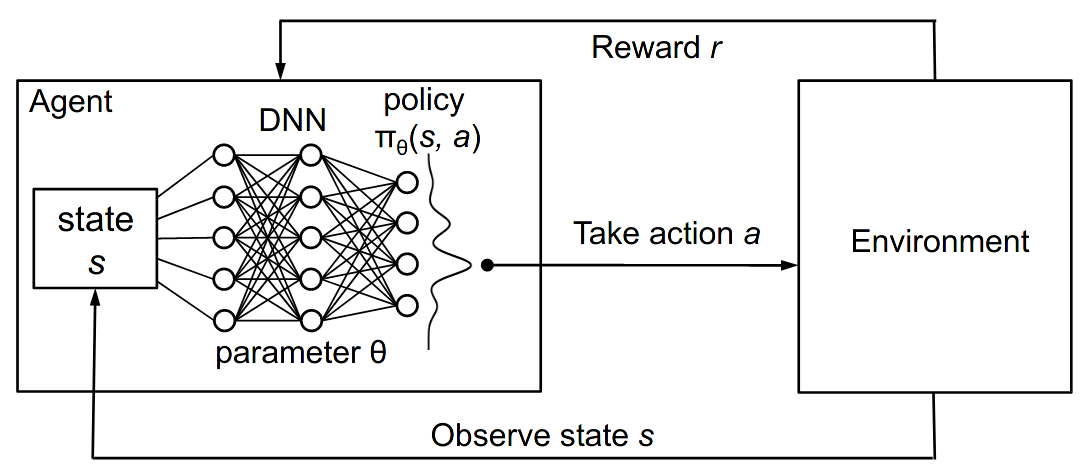
\includegraphics[scale=0.3]{DQN.png}\\
\end{figure}

\subsection{Actions Allowed}
The actions in this scenario, that is the DQN model, is the ordering of the operations we choose to execute. That is, we have $4 = 24$ possible actions on any given input. These are constructed using all possible permutations of $\{0,1,2,3\}$. We then transform this information into 1 hot encoding for ease of use.
\par Consider the set of permutations of $\{0,1,2,3\}$, we can order them lexicgraphically.\\
Given a permutation $\mathbb{P}$, it will have a rank $r$ in the ordering.\\
To convert the permutation into a $1$hot encoding, start with a $24$ element vector $v$ with all $0$s.Then update 
$$v[r]=1$$

\subsection{State Space}
We want the information extracted, i.e. the column wise entropy and the size of the relations, to represent the current state of the environment. Hence, any state is going to be represented as a vector of length $10$, the first $8$ are the column wise entropy and the $9^{th},10^{th}$ are the sizes of the two relations.\\
Note the makes the image of the state space to be a subset of $\mathbb{R}^{10}$. But as entropy is never going to be $0$ and so won't the size of the relations, we can trim it down to $(0,\infty)^{10}$ which is a continuous space.
\par Discretization is a process that divides numeric features into categorical  ones  using  intervals.   Depending  on  the  application and predictive model being used, discretization can bring several benefits, including faster computation time as discrete variables are usually easier to handle compared to numeric ones; and decreases the chances of overfitting since the feature space becomes less complex\cite{DNN_for_stream} . Targeting feature discretization from data streams, a significant milestone was the Partition Incremental Discretization algorithm (PiD)\cite{Pinto2005PartitionID}. While we have not used PiD, it is a powerful tool. PiD discretizes numeric features in two  layers.   The  first  layer  is  responsible  for  computing  a high number of intervals given the arriving data, while the second uses the statistics calculated in the first layer to compute equal frequency partitions.

\subsection{Reward System}
The reward system being used currently is simply taking the number of operations and time required(in micro seconds) as the reward. A more complex state will be when the rewards are not readily available, then another method can be applied as shown in \cite{know_unknown_rewards},\cite{DRL_rewards_problem}.\\
In traditional Q-learning, there is a discount factor involved to discount the moves done later on in the sequence of the game and there is a utility function involved to calculate the utility of each move for each state. The goal of the system is to maximize the expected utility.\\
As the game is a single move game, there is no discounting factor involved neither is a utility function required. We can use the negative of time required or the number of moves required to maximize or minimize with te current positive values. We chose to minimize the positive values.

\subsection{Transition function}
The transition function is the DQN, i.e. the reward determining system, along with the move choosing method. \\
The DQN will output a list of reward, which corresponds to the $24$ moves. Then to choose the optimal action based on reward, we simply scan a chunk of $24$ continuous rewards and associate them to moves.\\
As the game is a single state game, the model of DQN becomes rather simple, and makes it not necessary to choose a discount factor nor do we need to include it into the transition model.\\ 
The method to choose the optimal move is described in the next chapter formally.

\subsection{Assumptions}
Note the amount of information, features extracted from the querying do not fully represent the data set our Neural network can't perform very well. To tackle this, we look at whether the shift in the predicted rewards is similar cross all the moves.\\
Then given data points $(x_{i},y_{i}),(x_{j},y_{j})$ and the DQN $Q_{\theta}$ the condition to check becomes:-
$$y_{i}\leq y_{j}\Rightarrow Q_{\theta}(x_{i})\leq Q_{\theta}(x_{j})$$
If this condition holds, then the predicted optimal move is the actual optimal move. \\
As optimal move implies
$$y_{\text{optimal}}\leq y_{i} \forall i \in [24]$$
This with the previous condition will imply
$$Q_{\theta}(x_{\text{optimal}})\leq Q_{\theta}(x_{i})\forall i \in [24]$$ 
We train a Deep neural network with $70\%$, use the rest of the $30\%$ data for testing and record the results.


\section{Conclusion}
In this chapter we saw :- 
\begin{itemize}
    \item The method use to generate data for the linear road benchmark test cases.
    \item The method implemented to take input, converted $SQL$ queries to $C++$ and extracted features during execution and stored them
    \item Showcased how the extracted features can help with deep reinforcement learning
    \item Showcased the method used to evaluate the performance of DQN. 
\end{itemize}
In the next chapter, we
\begin{itemize}
    \item Formalize the assumptions we made in our evaulation.
    \item Present the categorize/ classification of the data set. Divided into training and testing data.
    \item Visualize the confusion matrix.
    \item Give the true positive, true negative, false positive false negative as well the analysis of the confusion matrix for all $24$ orderings.
    \item Lastly we compare how our predictions fared against the optimal and worst orderings. 
\end{itemize} present the results of our experiments, visualize them
 The method to compute the results are given in the next chapter.

\cleardoublepage

\chapter{Evaluation}
\label{chapter:evaluation}
\thispagestyle{myheadings}

% set this to the location of the figures for this chapter. it may
% also want to be ../Figures/2_Body/ or something. make sure that
% it has a trailing directory separator (i.e., '/')!
\graphicspath{{./5_Evaluation/}}

\section{Optimality checking}
Now we have learnt a model $Q_{\theta}$, we also have our test cases $\{(x_{i},y_{i})\}_{i\in[n]}$.\\
Each data window corresponds to $24$ data entries. The $t^{th}$ window corresponds to 
$$\{x_{24t}, x_{24t+1}, ..., x_{24t+23}|t\in\mathbb{I}\}$$
Each data window has $24$ data points as we have tried all possible($24$ of them) combinations of ordering of operations. For each data window we need to find the ordering of operations which requires the minimum moves according to our predictions.\\
To do this for the $t^{th}$ window of data, find the index of the minimum of $$Q_{\theta}(x_{24t}),Q_{\theta}(x_{24t+1}),...,Q_{\theta}(x_{24t+23})$$, say $k$.\\
To check if the move this corresponds to is the actual optimal move, find the index of the minimum of $y_{24t}, y_{24t+1}, ..., y_{24t+23}$, say $l$. If $k=l$ then the move we predicted as optimal is indeed optimal.\\ 
\par We train the model multiple times on the training data and measure its performance on the test data each time.\\
To measure the performance we use the predicted optimal move vs the actual optimal move.\\

\section{Justification}
The things considered while determining the neural network to use for training the DQN are :-
\begin{itemize}
    \item To achieve a value as close as possible to the global minima for the optimization function (Adam optimzer)
    \item The time required to predict the optimal move should not exceed the time saved by using it.
    \item The time and resources required for training should not exceed the capacity of the system while it is running the query processing in the background. 
\end{itemize}
What we found was:-
\begin{itemize}
    \item Adding additional layers improve the prediction of the optimal moves but not by significant margin.
    \item Adding additional layers resulted in the time spent predicting the answer overshadowing the time saved by executing the optimal move.
\end{itemize}
\par But note, these $2$ are only query and data specific findings.

\section{Results}
First, for each ordering of the operations we present the frequencies with which they are optimal in the dataset.
\begin{lstlisting}[caption=Frequencies of optimal moves in total data]
[0, 0, 0, 0, 0, 0, 0, 0, 0, 1, 0, 0, 110, 83, 84, 79, 80, 63, 307, 165, 2209, 1367, 43849, 43872]
\end{lstlisting} 
As visible the data is higly biased towards the last $2$ orderings.\\
We split this data into $70\%,30\%$ for the purpose of training and testing of our reinforcement learning agent.The random seed used resulted in the following split.
\begin{lstlisting}[caption= Frequencies of optimal move in training data]
[0, 0, 0, 0, 0, 0, 0, 0, 0, 0, 0, 0, 81, 60, 59, 54, 57, 45, 227, 119, 1526, 966, 30811, 30583]
\end{lstlisting}
\begin{lstlisting}[caption= Frequencies of optimal move in testing data]
[0, 0, 0, 0, 0, 0, 0, 0, 0, 1, 0, 0, 29, 23, 25, 25, 23, 18, 80, 46, 683, 401, 13038, 13289]
\end{lstlisting}
The predictions of our model resulted in the following $24$ true positive, False Positive, False negative and True negative results\\
\begin{lstlisting}[caption= True positives False positives False negatives True negatives]
(TP,FP,FN,TN)
(0.0, 0.0, 0.0, 27681.0)
(0.0, 0.0, 0.0, 27681.0)
(0.0, 0.0, 0.0, 27681.0)
(0.0, 0.0, 0.0, 27681.0)
(0.0, 0.0, 0.0, 27681.0)
(0.0, 0.0, 0.0, 27681.0)
(0.0, 0.0, 0.0, 27681.0)
(0.0, 0.0, 0.0, 27681.0)
(0.0, 0.0, 0.0, 27681.0)
(0.0, 0.0, 1.0, 27680.0)
(0.0, 0.0, 0.0, 27681.0)
(0.0, 0.0, 0.0, 27681.0)
(0.0, 0.0, 29.0, 27652.0)
(0.0, 3.0, 23.0, 27655.0)
(0.0, 0.0, 25.0, 27656.0)
(0.0, 0.0, 25.0, 27656.0)
(0.0, 0.0, 23.0, 27658.0)
(0.0, 0.0, 18.0, 27663.0)
(0.0, 7.0, 80.0, 27594.0)
(0.0, 0.0, 46.0, 27635.0)
(18.0, 251.0, 665.0, 26747.0)
(69.0, 973.0, 332.0, 26307.0)
(6347.0, 6789.0, 6691.0, 7854.0)
(6355.0, 6869.0, 6934.0, 7523.0)
\end{lstlisting}
So we got $12978$ predictions correct out of $27681$ test cases that is around $47\%$.
Below are 2 confusion matrices we obtained from two different runs of the predictions.\\

\begin{figure}
\caption{DQN Run 1 confusion matrix}
\centering
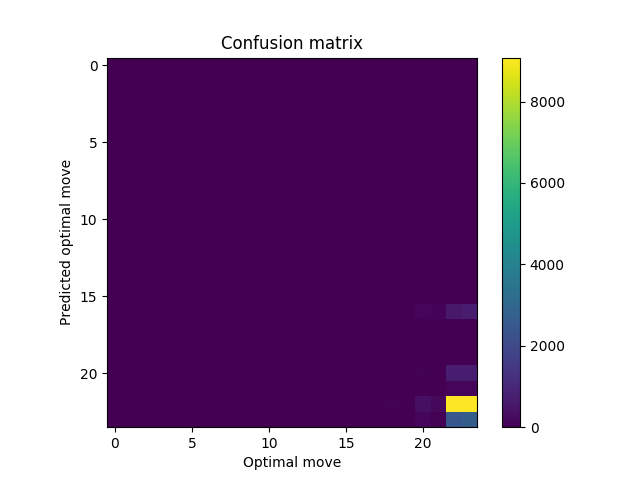
\includegraphics[scale=1]{cm1.png}\\
\end{figure}

\begin{figure}
\caption{DQN Run 1 confusion matrix closeup}
\centering
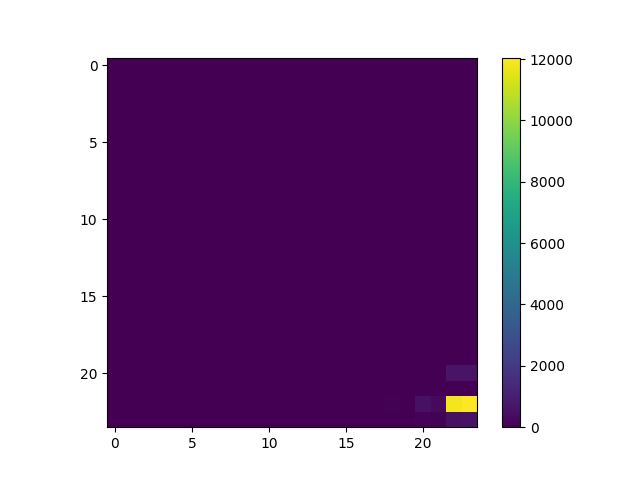
\includegraphics[scale=1]{cm2.png}\\
\end{figure}

\begin{figure}
\caption{DQN Run 2 confusion matrix}
\centering
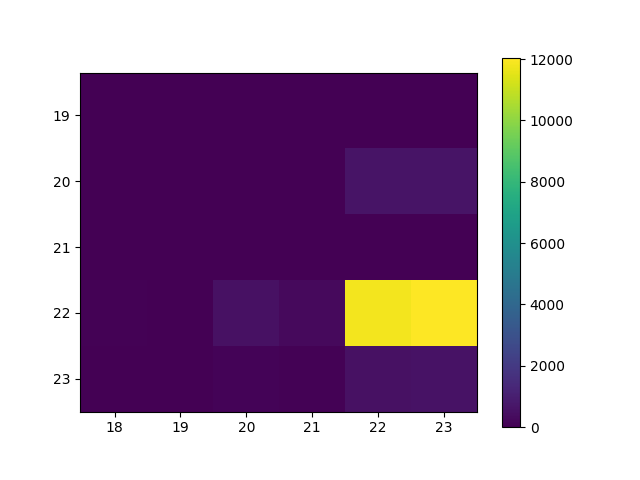
\includegraphics[scale=0.5]{cm3.png}\\
\end{figure}

\begin{figure}
\caption{DQN Run 2 confusion matrix closeup}
\centering
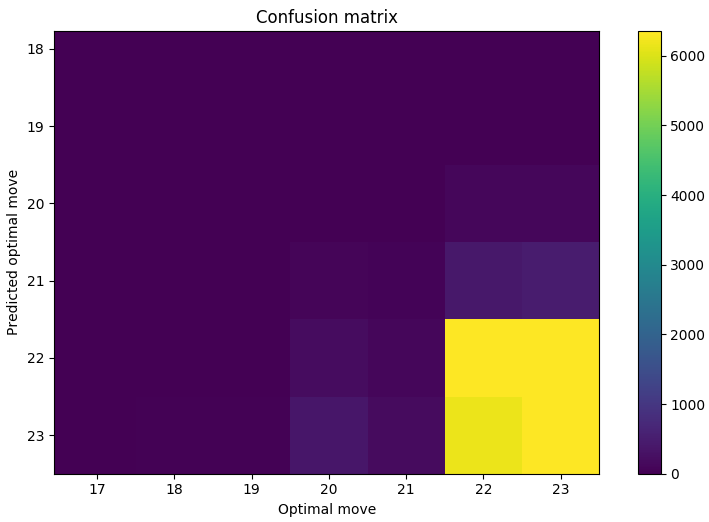
\includegraphics[scale=0.5]{cm4.png}\\
\end{figure}

Also have the actual confusion matrix for the second run.\\
\begin{lstlisting}[caption=Confusion matrix for DQN classificaiton]
[[   0    0    0    0    0    0    0    0    0    0    0    1    0]
 [   0    0    0    0    0    0    0    0    0    0    0   16   13]
 [   0    0    0    0    0    0    0    0    0    0    0   18    5]
 [   0    0    0    0    0    0    0    0    0    0    0   13   12]
 [   0    0    0    0    0    0    0    0    0    0    0   12   13]
 [   0    0    0    0    0    0    0    0    0    0    0   17    6]
 [   0    0    0    0    0    0    0    0    0    0    0    9    9]
 [   0    0    0    0    0    0    0    0    0    0   10   21   49]
 [   0    0    0    0    0    0    0    0    0    3    4   13   26]
 [   0    0    0    0    0    0    0    1    0   18   77  213  374]
 [   0    0    0    0    0    0    0    0    0   19   69  118  195]
 [   0    0    2    0    0    0    0    0    0  116  406 6347 6167]
 [   0    0    1    0    0    0    0    6    0  113  476 6338 6355]]
\end{lstlisting}
We have the actual optimal ordering, the actual worst ordering, the predicted best ordering from the model.\\
We add the number of operations required by following each of the above $3$ and look at the sum of them.\\
\begin{itemize}
    \item The sum of operations required by the optimal ordering $890640075.0$
    \item The sum of operations required by the predicted ordering $900269878.0$
    \item The sum of operations required by the optimal ordering $2310227856.0$
\end{itemize}
This tells us that our predicted orderings are approx $39\%$ of the worst ordering and $102\%$ of the best ordering.\\
A label based analysis is obtained by using $"\text{metrics.classification\_report}"$ from \\
 scikit-learn\cite{scikit-learn}.\\
\begin{lstlisting}[caption=Statistics for various orderings]
             precision    recall  f1-score   support

           9      0.000     0.000     0.000         1
          12      0.000     0.000     0.000        29
          13      0.000     0.000     0.000        23
          14      0.000     0.000     0.000        25
          15      0.000     0.000     0.000        25
          16      0.000     0.000     0.000        23
          17      0.000     0.000     0.000        18
          18      0.000     0.000     0.000        80
          19      0.000     0.000     0.000        46
          20      0.067     0.026     0.038       683
          21      0.066     0.172     0.096       401
          22      0.483     0.487     0.485     13038
          23      0.481     0.478     0.479     13289

   micro avg      0.462     0.462     0.462     27681
   macro avg      0.084     0.089     0.084     27681
weighted avg      0.461     0.462     0.461     27681
\end{lstlisting}

\section{Discussion}
\cite{DNN_for_stream} Learning from data streams is a continuous process. The learning systems that act in dynamic environments, where working conditions change and evolve, need to monitor their working conditions. They need to monitor the learning process  for change detection, emergence of novel classes, changes in the relevance of features, changes in the optimal parameters  settings, and others.\\
We divide this section into the following parts:-
\begin{itemize}
    \item \textbf{Interpretations} We will interpret the above stated results and see what they mean.
    \item \textbf{Implications} Why do these results matter and what can they lead to.
    \item \textbf{Limitations} the limitations we experienced in the experiments carried out in this thesis.
\end{itemize}


\subsection{Interpretations}
Despite the biased input data classes, the final strategy we got from the DQN gave us a performance of $101\%$ of the optimal solution, we can safely say, DQN have proved to be useful in this case. The successive epoches of DQN also can be seen to improve the results via the diagram.\\
But contrary to the expected result, the number of data points for which we were able to predict to optimal move correctly are roughly $48\%$, the lack of accuracy across the $24$ classes is concerning which can perhaps be addressed to the lack of features used in training the DQN.\\
Overall the improvement of optimal strategy selection is inline with the powerful nature of deep neural networks and iterative nature of reinforcement learning. The high amount of data available from data streams can definitely be a huge plus point for online training methods for DQN for query optimization.\\


\subsection{Implications}
The fact that the application of DQN improved performance by to such a margin, serves to prove that DQNs can be applied in at least some cases for optimizing queries on data stream. \cite{drl_dbms} Showcases method for using DQN for query optimization on  static data and we use it as an motivation to apply it on data streams.  \\
This makes a strong case for further work in this field, application of deep reinforcement learning to optimize query processing on stream data, to explore more SQL like implementation and integration of the DQN model along with online learning feature.\\
As we saw in this experiment, we achieved a model which tells us an strategy for ordering which requires only $1\%$ more operations than the optimal ordering. Application of DQN on other queries can similarly provide a huge speed up and perhaps reduction in resources consumed. \\
\cite{drl_dbms}It is popular in recent AI research to try end-to-end learning, where problems that were traditionally factored into subproblems (e.g., self-driving cars involve separate modelsfor localization, obstacle detection and lane-following) are learned in a single unified model. One can imagine a similar architectural ambition for an end-to-end learning query optimizer, which simply maps subplan features to measured runtimes. Thiis would require a significant corpus of run-time data to learn from, and changes to the featurization and perhaps the deep network structure we used here. DQ is a pragmatic middle ground that exploits the structure of the join optimization problem. 

\subsection{Limitations}
The work presented in this thesis has a number of limitations.
\begin{itemize}
    \item The neural network is unable to achieve low loss for the test data, this perhaps speak the the lack of features extracted during the querying time.
    \item The data sample we have is highly biased, leading to rather baised DQNs.
    \item The entire method need to be parallelized and set up on a scalable infrastructure to see the actual effects of DQN.
    \item The DQN used is simulating a single move game rather than a multi move game.
    \item Not looked at how DQNs can be trained online.
\end{itemize}


\section{Conclusion}
In this chapter we saw :-
\begin{itemize}
    \item The method for selecting the optimal move and the assumption for it.
    \item The classificaiton of the data and how it is split between training and testing.
    \item Analyzed and visualized the confusion matrix on different runs of DQN.
    \item The performance of the DQN on predicting.
\end{itemize}
In the next chapter we:-
\begin{itemize}
    \item Present the overall results of the thesis.
    \item Present the take aways.
    \item Present the ways of improving upon this work.
\end{itemize}
%1.2 change to research problem. Most important, 1.4
%Typing error, grammar

\cleardoublepage

\chapter{Conclusion and Further work}
\label{chapter:Conclusion_and_further_work}
\thispagestyle{myheadings}

% set this to the location of the figures for this chapter. it may
% also want to be ../Figures/2_Body/ or something. make sure that
% it has a trailing directory separator (i.e., '/')!
\graphicspath{}

\section{Conclusion}
The goal of this thesis is to act as a proof of concept for the application of Deep Reinforcement Learning for optimization of query processing on streams.\\
Say, for a particular window of data the size of SegVol $=x$ and size of SegAvgSpeed $=y$, due to the query used in the experiments, the number of operations required to execute the query lie between $[x*y,4*x*y]$. The worst and best possible cases can both arise in the same window depending on the order used and the data in the query.\\
Of the $24$ possible operation orders, we were able to predict the optimal order of operations around $48\%$ cases, reducing the number of operations to around $38\%$ of the worst observed(which is better than the actual worst).
\begin{center}
$x*y \leq$ optimal $\leq$ predicted $\leq$ worst observed $\leq 4*x*y$
\end{center}

\section{Further Work}
This thesis proposed a method for optimization of query execution on data stream and provided a demo implementation for experimentation. There are still many areas which can be improved and developed further.

\subsection{Data Generation}
As shown in chapter $5$, the data generated is highly biased. A source producing more diverse data and a query on that may lead to more interesting results. Real world data stream can be used to get better variety in the data and take input via different methods.

\subsection{Data Storage}
Currently, for executing the query, we store data in vectors where as SQL uses B-trees, a change like this can impact the time required for query execution and then lead to a different learnd model if the time of execution is used as reward.\\
On a further note data storage on systems like AWS S3 buckets, filesystems like Hadoop, hdfs and others can lead to changes in time of execution as well.

\subsection{Features extraction}
The current features only include the entropy of the columns and the size of the tables. Whereas in traditional SQL with a static database(relatively) a lot more features of generally extracted. Better starting feature can perhaps lead to a better results. 

\subsection{Deep Reinforcement Learning}
The Deep reinforcement learning model used was rather simplfied due to the less number of moves and convert the game into a single step game. Further intensive state, action and reward tuples can be constructed to get better intermediate rewards and policies. 

\subsection{Integration} 
The learnt DQN can be integrated with an actual stream processing system and tested in full for scalability, reliability and more. Need to note that there is a speedup by number of operations, the runtime due to various other network constraints might have a different result. 

\cleardoublepage



%\appendix
\begin{appendices}
\chapter{Proof of xyz}
\label{appendix}
\thispagestyle{myheadings}

This is the appendix.
\end{appendices}
%==========================================================================%
% Bibliography
\newpage
\singlespace
\bibliographystyle{apalike}

% each subdirectory can have its own BiBTeX file
\bibliography{thesis}
\cleardoublepage
%==========================================================================%
% Curriculum Vitae
\addcontentsline{toc}{chapter}{Curriculum Vitae}

\thispagestyle{empty}

\begin{center}
{\LARGE {\bf CURRICULUM VITAE}}\\
\vspace{0.5in}
{\large {\bf Joe Graduate}}
\end{center}

Basically, this needs to be worked out by each individual, however the same format, margins, typeface, and type size must be used as in the rest of the dissertation. 




%==========================================================================%
\end{document}


